% RECALL — english-vocabulary vault, practice set 4: comeback review (exercises)
% Compile with: pdflatex vocabulary-exercises-4.tex  (run twice)

\documentclass[11pt,a4paper]{article}
\usepackage[T1]{fontenc}
\usepackage[utf8]{inputenc}
\usepackage{charter}
\usepackage[scaled=0.92]{helvet}
\usepackage{courier}
\usepackage[safe]{tipa}
\usepackage{amssymb}
\usepackage{pifont}
\usepackage[a4paper,left=17mm,right=17mm,top=21mm,bottom=19mm,headsep=6mm,footskip=10mm]{geometry}
\usepackage{xcolor}
\usepackage{tikz}
\usetikzlibrary{calc,positioning,arrows.meta,backgrounds,shapes.geometric,shapes.misc,fit,decorations.pathreplacing,decorations.pathmorphing}
\usepackage[most]{tcolorbox}
\usepackage{enumitem}
\usepackage{multicol}
\usepackage{tabularx}
\usepackage{array}
\usepackage{booktabs}
\usepackage{colortbl}
\usepackage{fancyhdr}
\makeatletter
\newcommand{\needsp}[1]{\par\begingroup\setlength{\dimen@}{#1}\dimen@ii\pagegoal\advance\dimen@ii-\pagetotal
  \ifdim\dimen@>\dimen@ii\ifdim\dimen@ii>\z@\vfil\penalty-\@M\fi\fi\endgroup}
\makeatother
\raggedbottom
\usepackage{microtype}
\usepackage{etoolbox}
\usepackage{ragged2e}
\usepackage[hidelinks,pdftitle={Recall - Vocabulary vault comeback (exercises)},pdfauthor={FHX}]{hyperref}

% ---------- colours ----------
\definecolor{ink}{HTML}{1F2633}
\definecolor{inksoft}{HTML}{4A5466}
\definecolor{mute}{HTML}{8A93A3}
\definecolor{line}{HTML}{C3C9D4}
\definecolor{paper}{HTML}{F1F4F7}
\definecolor{accent}{HTML}{1C86C8}
\definecolor{accentdark}{HTML}{145E8E}
\definecolor{accentsoft}{HTML}{E3F0F9}
\definecolor{vault}{HTML}{E09F3E}
\definecolor{vaultsoft}{HTML}{FBF0DF}
\definecolor{good}{HTML}{2E8B57}
\definecolor{bad}{HTML}{C0392B}
% media colours (the shows your words came from)
\definecolor{mDB}{HTML}{E07A1F}
\definecolor{mJJK}{HTML}{6A4FC2}
\definecolor{mMHA}{HTML}{2E7D5B}
\definecolor{mMT}{HTML}{B5509A}
\definecolor{mDS}{HTML}{7A9A1F}
\definecolor{mPB}{HTML}{5A6170}
\definecolor{mFI}{HTML}{C8302C}
\definecolor{mLF}{HTML}{B07D12}
% voices (casters, chats)
\definecolor{vA}{HTML}{3A86C8}
\definecolor{vB}{HTML}{D1495B}

% ---------- fonts ----------
\newcommand{\mdot}{\ensuremath{\cdot}}
\newcommand{\arr}{\ensuremath{\rightarrow}}
\newcommand{\hfont}{\fontfamily{pag}\selectfont}
\newcommand{\uifont}{\sffamily}
\setlength{\parindent}{0pt}
\setlength{\parskip}{4pt}
\linespread{1.04}
\setlist{nosep,leftmargin=*}
\renewcommand{\arraystretch}{1.15}

% ---------- small TikZ icons (drawn in mm, centred on 0,0) ----------
\tikzset{
  ic/.style={x=1mm,y=1mm,line width=0.5pt,line join=round,line cap=round},
  pics/pencil/.style={code={
    \begin{scope}[rotate=40]
    \fill (-1.45,-0.32) rectangle (0.75,0.32);
    \fill (0.85,-0.32) -- (1.55,0) -- (0.85,0.32) -- cycle;
    \end{scope}}},
  pics/bubble/.style={code={
    \fill[rounded corners=0.55mm] (-1.5,-0.55) rectangle (1.5,1.05);
    \fill (-0.75,-0.45) -- (-1.05,-1.35) -- (-0.1,-0.45) -- cycle;}},
  pics/watch/.style={code={
    \draw (0,-0.2) circle (1.12);
    \fill (-0.28,0.95) rectangle (0.28,1.4);
    \draw (0,-0.2) -- (0,0.5);
    \draw (0,-0.2) -- (0.45,-0.2);}},
  pics/lens/.style={code={
    \draw[line width=0.62pt] (-0.35,0.35) circle (0.85);
    \draw[line width=1pt] (0.28,-0.28) -- (1.25,-1.25);}},
  pics/die/.style={code={
    \draw[rounded corners=0.35mm,line width=0.55pt] (-1.25,-1.25) rectangle (1.25,1.25);
    \fill (-0.6,0.6) circle (0.24); \fill (0.6,-0.6) circle (0.24); \fill (0,0) circle (0.24);}},
  pics/rewind/.style={code={
    \fill (-0.1,0) -- (1.3,0.95) -- (1.3,-0.95) -- cycle;
    \fill (-1.5,0) -- (-0.1,0.95) -- (-0.1,-0.95) -- cycle;}},
  pics/key/.style={code={
    \draw[line width=0.62pt] (-0.85,0.3) circle (0.62);
    \draw[line width=0.62pt] (-0.23,0.3) -- (1.55,0.3);
    \draw[line width=0.62pt] (1.05,0.3) -- (1.05,-0.35);
    \draw[line width=0.62pt] (1.5,0.3) -- (1.5,-0.2);}},
}
% mode icons: plain ink glyphs
\newcommand{\modeicon}[1]{\tikz[ic,baseline=-0.65ex]{\path (-1.9,-1.9) rectangle (1.9,1.9); \pic[inksoft] at (0,0) {#1};}}
\newcommand{\mWrite}{\modeicon{pencil}}
\newcommand{\mSpeak}{\modeicon{bubble}}
\newcommand{\mThink}{\modeicon{lens}}
\newcommand{\mTimed}{\modeicon{watch}}
\newcommand{\mDice}{\modeicon{die}}
% language chips
\newcommand{\langchip}[2]{\tikz[baseline=(c.base)]{\node[inner xsep=2.2pt,inner ysep=1.3pt,rounded corners=1.2pt,fill=#1,text=white,font=\uifont\bfseries\fontsize{6.2}{7}\selectfont](c){#2};}}
\newcommand{\PT}{\langchip{good}{PT}}
\newcommand{\UK}{\langchip{bad!85!ink}{UK}}
\newcommand{\US}{\langchip{accentdark}{US}}
% vault key marker
\newcommand{\vaultI}{\tikz[ic,baseline=-0.65ex]{\fill[vault] (0,0) circle (2.2); \pic[white,scale=0.85] at (0,0) {key};}}

% media chips: #1 colour, #2 label
\newcommand{\medchip}[2]{\tikz[baseline=(c.base)]{\node[inner xsep=1.8pt,inner ysep=0.9pt,rounded corners=1pt,fill=#1,text=white,font=\uifont\bfseries\fontsize{5.6}{6}\selectfont](c){#2};}}
\newcommand{\mDBZ}{\medchip{mDB}{DBZ}}
\newcommand{\mDBS}{\medchip{mDB}{DBS}}
\newcommand{\mGT}{\medchip{mDB}{GT}}
\newcommand{\mJJK}{\medchip{mJJK}{JJK}}
\newcommand{\mMHA}{\medchip{mMHA}{MHA}}
\newcommand{\mMT}{\medchip{mMT}{MT}}
\newcommand{\mDS}{\medchip{mDS}{DS}}
\newcommand{\mPB}{\medchip{mPB}{PB}}
\newcommand{\mFI}{\medchip{mFI}{F1}}
\newcommand{\mLF}{\medchip{mLF}{LIFE}}

% ---------- slanted label (Overwatch-HUD style parallelogram) ----------
% #1 half-slant, #2 fill colour, #3 node options, #4 text
\newcommand{\slant}[4][2.2pt]{\tikz[baseline=(t.base)]{\node[inner xsep=5pt,inner ysep=2.4pt,#3](t){#4};
  \begin{scope}[on background layer]\fill[#2]($(t.south west)+(-#1,0)$)--($(t.south east)+(-#1,0)$)--($(t.north east)+(#1,0)$)--($(t.north west)+(#1,0)$)--cycle;\end{scope}}}
% knowledge tags
\newcommand{\tg}[1]{\slant[1.5pt]{ink!9}{font=\hfont\bfseries\scriptsize,text=inksoft,inner xsep=3.2pt,inner ysep=1.6pt}{#1}}
\newcommand{\tgA}[1]{\slant[1.3pt]{ink!8}{font=\hfont\bfseries\tiny,text=inksoft,inner xsep=2.3pt,inner ysep=1.2pt}{#1}}
\newcommand{\tgL}[2]{\slant[1.5pt]{ink!9}{font=\hfont\scriptsize,text=inksoft,inner xsep=3.2pt,inner ysep=1.6pt}{\textbf{#1}\,{\color{mute}·}\,#2}}
\newcommand{\exnum}[1]{\slant[3pt]{accent}{font=\hfont\bfseries\fontsize{19}{19}\selectfont,text=white,inner xsep=7pt,inner ysep=5pt,minimum height=10.5mm}{#1}}

% ---------- headers / footers ----------
\setlength{\headheight}{14pt}
\pagestyle{fancy}
\fancyhf{}
\renewcommand{\headrulewidth}{0.4pt}
\renewcommand{\headrule}{{\color{line}\hrule height 0.4pt}}
\fancyhead[L]{{\hfont\bfseries\footnotesize\color{accent}RECALL}{\hfont\footnotesize\color{mute}\ \ \mdot{}\ \ Vocabulary vault comeback}}
\fancyhead[R]{{\hfont\footnotesize\color{mute}Exercises}}
\fancyfoot[R]{\slant[2pt]{ink}{font=\hfont\bfseries\footnotesize,text=white,inner xsep=6pt}{\thepage}}
\fancyfoot[L]{{\hfont\scriptsize\color{mute}english-vocabulary vault \mdot{}\ Practice set 4}}
\fancypagestyle{plain}{\fancyhf{}\renewcommand{\headrulewidth}{0pt}\fancyfoot[R]{\slant[2pt]{ink}{font=\hfont\bfseries\footnotesize,text=white,inner xsep=6pt}{\thepage}}}

% ---------- part banner ----------
% #1 part label, #2 title, #3 subtitle
\newcommand{\partbanner}[3]{%
  \needsp{100mm}\vspace{6mm}
  \noindent\begin{tikzpicture}
    \path[use as bounding box] (0,0) rectangle (\linewidth,-21.5mm);
    \fill[ink] (0,0) -- (\linewidth,0) -- (\linewidth-9mm,-15mm) -- (0,-15mm) -- cycle;
    \fill[accent] (0,0) rectangle (3.2mm,-15mm);
    \fill[accent] (\linewidth-5mm,0) -- (\linewidth,0) -- (\linewidth-9mm,-15mm) -- (\linewidth-14mm,-15mm) -- cycle;
    \fill[vault] (\linewidth-12mm,0) -- (\linewidth-9.6mm,0) -- (\linewidth-18.6mm,-15mm) -- (\linewidth-21mm,-15mm) -- cycle;
    \node[anchor=west,font=\hfont\bfseries\footnotesize,text=accent!70!white] at (7.5mm,-4.6mm) {#1};
    \node[anchor=west,font=\hfont\bfseries\fontsize{21}{23}\selectfont,text=white] at (7mm,-10.3mm) {#2};
    \node[anchor=north west,font=\itshape\small,text=inksoft,inner sep=0pt] at (0.4mm,-17.6mm) {#3};
  \end{tikzpicture}\par\vspace{1mm}}

% ---------- exercise header ----------
% #1 number, #2 title, #3 tag pills, #4 icons
\newcommand{\exhead}[5][10\baselineskip]{%
  \needsp{#1}\vspace{9pt}%
  \noindent\begin{tikzpicture}[baseline=(n.south)]
    \node[anchor=south west,inner sep=0pt] (n) at (0,0) {\exnum{#2}};
    \node[anchor=south west,inner sep=0pt,font=\hfont\bfseries\fontsize{14.5}{16}\selectfont,text=ink] (t) at ($(n.south east)+(4mm,4.8mm)$) {#3};
    \node[anchor=south west,inner sep=0pt] (u) at ($(n.south east)+(4mm,0.1mm)$) {#4};
    \node[anchor=south east,inner sep=0pt] (i) at (\linewidth-0.3pt,1.2mm) {#5};
    \draw[line,line width=0.6pt] (0.3pt,-1.6mm) -- (\linewidth-0.3pt,-1.6mm);
  \end{tikzpicture}\par\vspace{3pt}}
\newcommand{\instr}[1]{{\small\color{inksoft}#1}\par\vspace{2pt}}

% ---------- gaps, options, writing lines ----------
% #1 number, #2 width, #3 hint
\newcommand{\gap}[3]{\mbox{{\uifont\bfseries\scriptsize\color{accent}#1}\kern1.2pt\textcolor{mute}{\rule[-0.5ex]{#2}{0.5pt}}}\ifstrempty{#3}{}{\ ({\itshape #3})}}
\newcommand{\opt}[2]{\mbox{{\color{mute}[}\,{\uifont\small #1}~{\color{mute}/}~{\uifont\small #2}\,{\color{mute}]}}}
\newcommand{\optt}[3]{\mbox{{\color{mute}[}\,{\uifont\small #1}~{\color{mute}/}~{\uifont\small #2}~{\color{mute}/}~{\uifont\small #3}\,{\color{mute}]}}}
\newcommand{\wfill}{\leavevmode{\color{line}\leaders\hrule height 0.5pt\hfill\kern0pt}}
\newcommand{\wline}{\par\vspace{5.6mm}\noindent{\color{line}\rule{\linewidth}{0.5pt}}\par}
\newcommand{\wlines}[1]{\foreach\x in {1,...,#1}{\wline}\vspace{1mm}}
\newcommand{\num}[1]{\leavevmode{\uifont\bfseries\small\color{accent}#1}}
\newcommand{\blank}[1][1.25cm]{\textcolor{mute}{\rule[-0.45ex]{#1}{0.5pt}}}
\newcommand{\cbox}{\tikz[baseline=-0.75ex]{\draw[mute,line width=0.5pt,rounded corners=0.4pt] (0,-1.35mm) rectangle (2.7mm,1.35mm);}}
\newcommand{\lbox}[1]{\tikz[baseline=-0.75ex]{\draw[mute,line width=0.5pt,rounded corners=0.4pt] (0,-1.6mm) rectangle (#1,1.6mm);}}
\newcommand{\hl}[1]{{\uifont\bfseries #1}}
\newcommand{\sout}[1]{\tikz[baseline=(t.base)]{\node[inner sep=0pt,text=inksoft](t){#1}; \draw[bad,line width=0.7pt] ([xshift=-0.4pt]t.mid west) -- ([xshift=0.4pt]t.mid east);}}
\newcommand{\ul}[1]{\underline{#1}}
\newcommand{\word}[1]{{\uifont\bfseries\color{ink}#1}}

% ---------- boxes ----------
\newtcolorbox{infobox}[2][]{enhanced,breakable,colback=paper,colframe=paper,boxrule=0pt,arc=2mm,left=4mm,right=4mm,top=3mm,bottom=3mm,
  fonttitle=\hfont\bfseries\small,coltitle=ink,title={#2},attach title to upper={\par\vspace{2pt}},#1}
\newtcolorbox{vocabbox}[2][]{enhanced,breakable,colback=white,colframe=#1,boxrule=0.6pt,arc=2mm,left=4mm,right=4mm,top=2.5mm,bottom=2.5mm,
  fonttitle=\hfont\bfseries\small,coltitle=#1,title={#2},attach title to upper={\par\vspace{1pt}},fontupper=\small}
\newtcolorbox{speakbox}[1][]{enhanced,breakable,colback=accentsoft,colframe=accentsoft,boxrule=0pt,arc=2mm,left=4mm,right=4mm,top=2.5mm,bottom=2.5mm,
  fontupper=\small,#1}
\newtcolorbox{vaultbox}[1][]{enhanced,breakable,colback=vaultsoft,colframe=vaultsoft,boxrule=0pt,arc=2mm,left=4mm,right=4mm,top=2.5mm,bottom=2.5mm,
  fontupper=\small,#1}
\newcommand{\banksep}{}
\newcommand{\bankitem}[1]{\banksep\mbox{#1}\gdef\banksep{\nobreak\hspace{0.5em plus 0.3em}{\color{mute}\mdot}\nobreak\hspace{0.5em plus 0.3em}\allowbreak}}
\newcommand{\bank}[1]{\gdef\banksep{}\forcsvlist{\bankitem}{#1}}
\newtcolorbox{wordbank}[1][]{enhanced,colback=white,colframe=line,boxrule=0.5pt,arc=1.5mm,left=3mm,right=3mm,top=1.6mm,bottom=1.6mm,
  fontupper=\small\uifont,halign=center,#1}

% tier badge: #1 colour, #2 letter
\newcommand{\tier}[2]{\tikz[baseline=(t.base)]{\node[inner sep=0pt,minimum width=7mm,minimum height=6.2mm,font=\hfont\bfseries\large,text=white](t){#2};
  \begin{scope}[on background layer]\fill[#1]($(t.south west)+(-1.2pt,0)$)--($(t.south east)+(-1.2pt,0)$)--($(t.north east)+(1.2pt,0)$)--($(t.north west)+(1.2pt,0)$)--cycle;\end{scope}}}

\begin{document}

\thispagestyle{plain}
\noindent
\begin{tikzpicture}
  \path[use as bounding box] (0,0) rectangle (\linewidth,-47mm);
  \fill[ink] (0,0) -- (\linewidth,0) -- (\linewidth-14mm,-41mm) -- (0,-41mm) -- cycle;
  \fill[accent] (\linewidth-7mm,0) -- (\linewidth,0) -- (\linewidth-14mm,-41mm) -- (\linewidth-21mm,-41mm) -- cycle;
  \fill[vault] (\linewidth-17mm,0) -- (\linewidth-13.5mm,0) -- (\linewidth-27.5mm,-41mm) -- (\linewidth-31mm,-41mm) -- cycle;
  \fill[accent] (0,0) rectangle (3.6mm,-41mm);
  \node[anchor=west,font=\hfont\bfseries\footnotesize,text=accent!75!white] at (9mm,-8mm) {ENGLISH-VOCABULARY VAULT \enspace\mdot{}\enspace 925 CARDS \enspace\mdot{}\enspace COMEBACK REVIEW};
  \node[anchor=west,font=\hfont\bfseries\fontsize{52}{54}\selectfont,text=white] (T) at (7.5mm,-21.5mm) {RECALL};
  \node[anchor=west] at ([xshift=5mm,yshift=1mm]T.east) {\tikz[x=1mm,y=1mm]{\fill[accent] (-0.1,0) -- (5.2,3.8) -- (5.2,-3.8) -- cycle; \fill[accent] (-5.6,0) -- (-0.1,3.8) -- (-0.1,-3.8) -- cycle;}};
  \node[anchor=west,font=\hfont\large,text=white!82!ink] at (9mm,-33mm) {Rewind the vault. Get the words back on your tongue.};
\end{tikzpicture}
\par\vspace{1mm}
{\small\color{inksoft}The words worth keeping from \emph{Dragon Ball}, \emph{Jujutsu Kaisen Modulo}, \emph{My Hero Academia Vigilantes}, \emph{Mushoku Tensei}, \emph{Dr.\ Stone} and the rest of your vault — meanings, forgotten senses, phrasal verbs, idioms, register and British English — mixed the way you will actually meet them: in Leuven, on Discord, in the lab and in the news.}
\vspace{3mm}

\noindent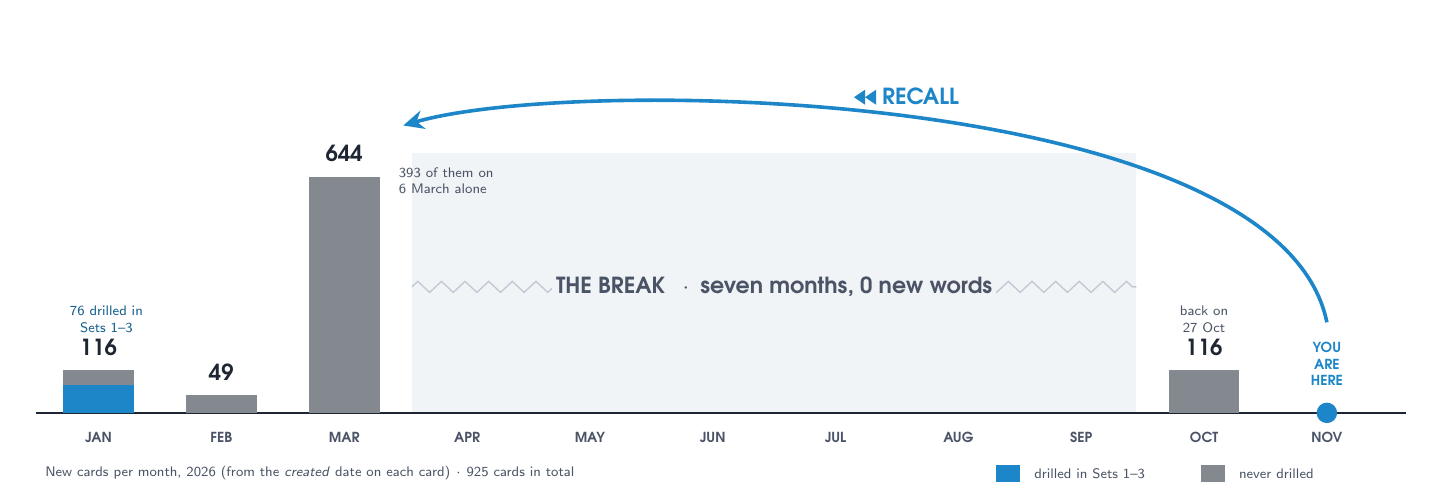
\begin{tikzpicture}[x=1mm,y=1mm,font=\uifont\scriptsize]
\path[use as bounding box] (-1,-11) rectangle (175,44);
\fill[paper] (47.80,0) rectangle (139.80,33);
\draw[line,line width=0.5pt,decorate,decoration={zigzag,segment length=3mm,amplitude=0.7mm}] (47.80,16) -- (139.80,16);
\node[fill=paper,inner sep=1.5pt,font=\hfont\bfseries\footnotesize,text=inksoft] at (93.80,16) {THE BREAK \enspace\mdot\enspace seven months, 0 new words};
\draw[ink,line width=0.6pt] (0,0) -- (174,0);
\node[anchor=north,font=\hfont\bfseries\tiny,text=inksoft] at (8.00,-1.2) {JAN};
\fill[accent] (3.50,0) rectangle (12.50,3.54);
\fill[ink!55] (3.50,3.54) rectangle (12.50,5.40);
\node[anchor=south,font=\hfont\bfseries\footnotesize,text=ink] at (8.00,6.00) {116};
\node[anchor=north,font=\hfont\bfseries\tiny,text=inksoft] at (23.60,-1.2) {FEB};
\fill[ink!55] (19.10,0) rectangle (28.10,2.28);
\node[anchor=south,font=\hfont\bfseries\footnotesize,text=ink] at (23.60,2.88) {49};
\node[anchor=north,font=\hfont\bfseries\tiny,text=inksoft] at (39.20,-1.2) {MAR};
\fill[ink!55] (34.70,0) rectangle (43.70,30.00);
\node[anchor=south,font=\hfont\bfseries\footnotesize,text=ink] at (39.20,30.60) {644};
\node[anchor=north,font=\hfont\bfseries\tiny,text=inksoft] at (54.80,-1.2) {APR};
\node[anchor=north,font=\hfont\bfseries\tiny,text=inksoft] at (70.40,-1.2) {MAY};
\node[anchor=north,font=\hfont\bfseries\tiny,text=inksoft] at (86.00,-1.2) {JUN};
\node[anchor=north,font=\hfont\bfseries\tiny,text=inksoft] at (101.60,-1.2) {JUL};
\node[anchor=north,font=\hfont\bfseries\tiny,text=inksoft] at (117.20,-1.2) {AUG};
\node[anchor=north,font=\hfont\bfseries\tiny,text=inksoft] at (132.80,-1.2) {SEP};
\node[anchor=north,font=\hfont\bfseries\tiny,text=inksoft] at (148.40,-1.2) {OCT};
\fill[ink!55] (143.90,0) rectangle (152.90,5.40);
\node[anchor=south,font=\hfont\bfseries\footnotesize,text=ink] at (148.40,6.00) {116};
\node[anchor=north,font=\hfont\bfseries\tiny,text=inksoft] at (164.00,-1.2) {NOV};
\node[anchor=west,text=inksoft,align=left,font=\uifont\tiny] at (44.90,29.5) {393 of them on\\6 March alone};
\node[anchor=south,text=accentdark,align=center,font=\uifont\tiny] at (9.00,9.0) {76 drilled in\\Sets 1--3};
\node[anchor=south,text=inksoft,align=center,font=\uifont\tiny] at (148.40,9.0) {back on\\27 Oct};
\fill[accent] (164.00,0) circle (1.3);
\node[anchor=south,text=accent,font=\hfont\bfseries\tiny,align=center] at (164.00,2.2) {YOU\\ARE\\HERE};
\draw[accent,line width=1.3pt,-{Stealth[length=2.6mm,width=2.4mm]}] (164.00,11.5) .. controls (158.00,41) and (69.20,43) .. (46.70,36.5);
\node[fill=white,inner sep=1.2pt,text=accent,font=\hfont\bfseries\footnotesize] at (110.60,40.2) {\tikz[ic,baseline=-0.6ex]{\pic[accent] at (0,0) {rewind};}\ RECALL};
\fill[accent] (122,-8.8) rectangle (125,-6.6); \node[anchor=west,text=inksoft,font=\uifont\tiny] at (125.6,-7.7) {drilled in Sets 1--3};
\fill[ink!55] (148,-8.8) rectangle (151,-6.6); \node[anchor=west,text=inksoft,font=\uifont\tiny] at (151.6,-7.7) {never drilled};
\node[anchor=west,text=inksoft,font=\uifont\tiny] at (0,-7.7) {New cards per month, 2026 (from the \textit{created} date on each card) \mdot\ 925 cards in total};
\end{tikzpicture}
\par\vspace{2.5mm}
\noindent{\hfont\bfseries\scriptsize\color{ink}WHERE THE 925 CARDS CAME FROM}\par\vspace{1mm}
\noindent
\begin{tikzpicture}[x=1mm,y=1mm,font=\uifont\scriptsize]
\fill[mDB] (0.00,0) rectangle (96.88,6);
\node[text=white,font=\hfont\bfseries\tiny] at (48.44,3) {DBZ \enspace 515};
\fill[mJJK] (96.88,0) rectangle (140.52,6);
\node[text=white,font=\hfont\bfseries\tiny] at (118.70,3) {JJK \enspace 232};
\fill[mMHA] (140.52,0) rectangle (154.06,6);
\node[text=white,font=\hfont\bfseries\tiny] at (147.29,3) {MHA \enspace 72};
\fill[mMT] (154.06,0) rectangle (162.34,6);
\fill[mDB!70!white] (162.34,0) rectangle (167.42,6);
\fill[mDS] (167.42,0) rectangle (170.80,6);
\fill[mDB!45!white] (170.80,0) rectangle (172.12,6);
\fill[mLF] (172.12,0) rectangle (173.06,6);
\fill[mPB] (173.06,0) rectangle (173.81,6);
\fill[mFI] (173.81,0) rectangle (174.00,6);
\node[anchor=north west,text=inksoft,font=\uifont\tiny,inner sep=0pt] at (0,-1.6) {DBZ = Dragon Ball Z, JJK = Jujutsu Kaisen Modulo, MHA = My Hero Academia Vigilantes \enspace\mdot\enspace smaller slices: \textcolor{mMT}{\textbf{MT}} 44 \enspace\mdot\enspace \textcolor{mDB}{\textbf{DBS}} 27 \enspace\mdot\enspace \textcolor{mDS}{\textbf{DS}} 18 \enspace\mdot\enspace \textcolor{mDB}{\textbf{GT}} 7 \enspace\mdot\enspace \textcolor{mLF}{\textbf{LIFE}} 5 \enspace\mdot\enspace \textcolor{mPB}{\textbf{PB}} 4 \enspace\mdot\enspace \textcolor{mFI}{\textbf{F1}} 1};
\end{tikzpicture}
\par\vspace{6mm}

\begin{infobox}{HOW THIS REVIEW WORKS}
\begin{enumerate}[label={\hfont\bfseries\color{accent}\arabic*},leftmargin=6mm,itemsep=2.4pt]
\item \textbf{Retrieve, don’t re-read.} Closed book: no vault, no dictionary, no key until you have finished a part. The effort of dragging a word out of memory is exactly what makes it stay.
\item \textbf{Say it out loud.} Before you write an answer, say the whole sentence at normal speed. The stutter disappears in your mouth, not on paper.
\item \textbf{Use your colours.} {\color{accent}\textbf{Blue}} = right first time, {\color{vault}\textbf{orange}} = small slip, {\color{bad}\textbf{red}} = wrong, then corrected.
\item \textbf{Tag your reds.} Every answer in the key carries a tag (\tgA{C}\,=\,collocation, \tgA{P}\,=\,phrasal verbs \ldots). On the \emph{Rundown} page, colour one square per red: your hottest rows tell you what to revisit.
\item \textbf{Three sessions, not a marathon.} Parts 1--3 \arr{} Parts 4--5 \arr{} Parts 6--7 + Rundown. After that, the rematch schedule on the last page takes over.
\end{enumerate}
\end{infobox}
\vspace{1mm}
\noindent{\hfont\bfseries\small\color{ink}ICONS}\par\vspace{0.6mm}
\noindent{\small\mWrite~Write \quad \mSpeak~Speak \quad \mThink~Think / puzzle \quad \mTimed~Timed \quad \mDice~Dice \quad \PT~uses your Portuguese \quad \UK~British English}

\newpage
\noindent\slant[2.4pt]{ink}{font=\hfont\bfseries\normalsize,text=white,inner xsep=7pt,inner ysep=3.4pt}{BRIEFING}\hspace{3mm}{\hfont\bfseries\large\color{ink}What a seven-month break does to 925 words}
\par\vspace{2mm}
\begin{enumerate}[label={\hfont\bfseries\color{accent}\arabic*},leftmargin=6mm,itemsep=3pt]
\item \textbf{Recognition outlives recall.} You will still \emph{recognise} most of your words when you see them. What fades first is pulling them out on demand — in a seminar, on Discord, in a lab report. That is the stutter. So almost every exercise here makes you \emph{produce} the word, not just spot it.
\item \textbf{Chunks fall apart.} Fluency lives in ready-made chunks — \emph{pay through the nose}, \emph{chip away at}, \emph{be that as it may}. After a break they come back with the wrong particle or a missing word. Parts 4 and 5 rebuild them.
\item \textbf{Senses collapse.} Words with several meanings shrink back to the first one you met (usually the anime one): \emph{floor, coast, toll, strain}\ldots{} Part 2 brings the other meanings back.
\item \textbf{Your vault speaks American.} Most of it came from US dubs and subtitles — but you study British English. Part 6 converts.
\item \textbf{Not all 925 deserve equal time.} 644 cards entered the vault in three days of March and were never drilled. Nobody keeps that many from a single pass, so this review \emph{triages}.
\end{enumerate}
\vspace{2mm}

\noindent{\hfont\bfseries\small\color{ink}THE TRIAGE}\enspace{\small\color{inksoft}— how the words in this review were chosen}\par\vspace{1.5mm}
\noindent\begin{tabularx}{\linewidth}{@{}m{9mm}@{}>{\RaggedRight\arraybackslash}m{37mm}>{\RaggedRight\arraybackslash\small}X@{}}
\tier{accent}{S} & {\hfont\bfseries\small Use it}\newline{\footnotesize\color{inksoft}at uni and in real life} & Formal power words and discourse chunks: \emph{assess, convey, deem, hinder, withhold, scrutiny, inherently, be that as it may, at the expense of}\ldots\\[2.2mm]
\tier{accent!55}{A} & {\hfont\bfseries\small Sound natural}\newline{\footnotesize\color{inksoft}talk, Discord, gaming} & Phrasal verbs, idioms and people words: \emph{pull off, chip away at, call it quits, turn a blind eye, a blessing in disguise, gullible, stuck-up}\ldots\\[2.2mm]
\tier{mute}{B} & {\hfont\bfseries\small Recognise it}\newline{\footnotesize\color{inksoft}reading and watching} & Dramatic, fantasy-flavoured words: \emph{foreboding, wrath, onslaught, perish, smithereens, envoy, decree}\ldots\\[2.2mm]
\tier{line}{C} & {\hfont\bfseries\small Let it go}\newline{\footnotesize\color{inksoft}no drilling needed} & Dub-only slang, cartoon insults, archaic or ultra-specific words: \emph{tarnation, oogey, whippersnapper, doughboy, cruller, cephalopod, thee}\ldots\\
\end{tabularx}
\par\vspace{1.5mm}
{\small This review drills tiers S and A, gives B a light touch and leaves C on the bench. The full \emph{let-it-go} list is on the last page — permission granted.}
\vspace{4mm}

\noindent{\hfont\bfseries\small\color{ink}WHAT EACH EXERCISE TRAINS}\enspace{\small\color{inksoft}(a dot = that kind of knowledge is tested there)}\par\vspace{2mm}
\begin{center}
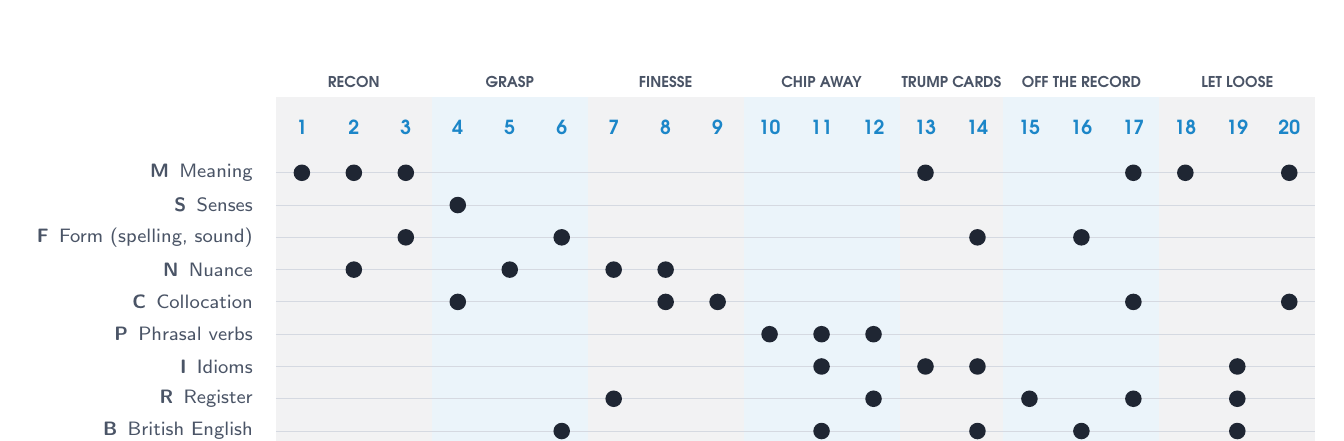
\begin{tikzpicture}[x=1mm,y=-1mm,font=\uifont\scriptsize]
\fill[ink!6] (37.70,-7.4) rectangle (57.50,37.60);
\node[font=\hfont\bfseries\fontsize{5.4}{6}\selectfont,text=inksoft] at (47.60,-9.4) {RECON};
\fill[accent!9] (57.50,-7.4) rectangle (77.30,37.60);
\node[font=\hfont\bfseries\fontsize{5.4}{6}\selectfont,text=inksoft] at (67.40,-9.4) {GRASP};
\fill[ink!6] (77.30,-7.4) rectangle (97.10,37.60);
\node[font=\hfont\bfseries\fontsize{5.4}{6}\selectfont,text=inksoft] at (87.20,-9.4) {FINESSE};
\fill[accent!9] (97.10,-7.4) rectangle (116.90,37.60);
\node[font=\hfont\bfseries\fontsize{5.4}{6}\selectfont,text=inksoft] at (107.00,-9.4) {CHIP AWAY};
\fill[ink!6] (116.90,-7.4) rectangle (130.10,37.60);
\node[font=\hfont\bfseries\fontsize{5.4}{6}\selectfont,text=inksoft] at (123.50,-9.4) {TRUMP CARDS};
\fill[accent!9] (130.10,-7.4) rectangle (149.90,37.60);
\node[font=\hfont\bfseries\fontsize{5.4}{6}\selectfont,text=inksoft] at (140.00,-9.4) {OFF THE RECORD};
\fill[ink!6] (149.90,-7.4) rectangle (169.70,37.60);
\node[font=\hfont\bfseries\fontsize{5.4}{6}\selectfont,text=inksoft] at (159.80,-9.4) {LET LOOSE};
\node[font=\hfont\bfseries\scriptsize,text=accent] at (41.00,-3.6) {1};
\node[font=\hfont\bfseries\scriptsize,text=accent] at (47.60,-3.6) {2};
\node[font=\hfont\bfseries\scriptsize,text=accent] at (54.20,-3.6) {3};
\node[font=\hfont\bfseries\scriptsize,text=accent] at (60.80,-3.6) {4};
\node[font=\hfont\bfseries\scriptsize,text=accent] at (67.40,-3.6) {5};
\node[font=\hfont\bfseries\scriptsize,text=accent] at (74.00,-3.6) {6};
\node[font=\hfont\bfseries\scriptsize,text=accent] at (80.60,-3.6) {7};
\node[font=\hfont\bfseries\scriptsize,text=accent] at (87.20,-3.6) {8};
\node[font=\hfont\bfseries\scriptsize,text=accent] at (93.80,-3.6) {9};
\node[font=\hfont\bfseries\scriptsize,text=accent] at (100.40,-3.6) {10};
\node[font=\hfont\bfseries\scriptsize,text=accent] at (107.00,-3.6) {11};
\node[font=\hfont\bfseries\scriptsize,text=accent] at (113.60,-3.6) {12};
\node[font=\hfont\bfseries\scriptsize,text=accent] at (120.20,-3.6) {13};
\node[font=\hfont\bfseries\scriptsize,text=accent] at (126.80,-3.6) {14};
\node[font=\hfont\bfseries\scriptsize,text=accent] at (133.40,-3.6) {15};
\node[font=\hfont\bfseries\scriptsize,text=accent] at (140.00,-3.6) {16};
\node[font=\hfont\bfseries\scriptsize,text=accent] at (146.60,-3.6) {17};
\node[font=\hfont\bfseries\scriptsize,text=accent] at (153.20,-3.6) {18};
\node[font=\hfont\bfseries\scriptsize,text=accent] at (159.80,-3.6) {19};
\node[font=\hfont\bfseries\scriptsize,text=accent] at (166.40,-3.6) {20};
\node[anchor=east,text=inksoft] at (36.00,2.20) {\textbf{M}\enspace Meaning};
\draw[line!70,line width=0.3pt] (37.70,2.20) -- (169.70,2.20);
\fill[ink] (41.00,2.20) circle (1.05);
\fill[ink] (47.60,2.20) circle (1.05);
\fill[ink] (54.20,2.20) circle (1.05);
\fill[ink] (120.20,2.20) circle (1.05);
\fill[ink] (146.60,2.20) circle (1.05);
\fill[ink] (153.20,2.20) circle (1.05);
\fill[ink] (166.40,2.20) circle (1.05);
\node[anchor=east,text=inksoft] at (36.00,6.30) {\textbf{S}\enspace Senses};
\draw[line!70,line width=0.3pt] (37.70,6.30) -- (169.70,6.30);
\fill[ink] (60.80,6.30) circle (1.05);
\node[anchor=east,text=inksoft] at (36.00,10.40) {\textbf{F}\enspace Form (spelling, sound)};
\draw[line!70,line width=0.3pt] (37.70,10.40) -- (169.70,10.40);
\fill[ink] (54.20,10.40) circle (1.05);
\fill[ink] (74.00,10.40) circle (1.05);
\fill[ink] (126.80,10.40) circle (1.05);
\fill[ink] (140.00,10.40) circle (1.05);
\node[anchor=east,text=inksoft] at (36.00,14.50) {\textbf{N}\enspace Nuance};
\draw[line!70,line width=0.3pt] (37.70,14.50) -- (169.70,14.50);
\fill[ink] (47.60,14.50) circle (1.05);
\fill[ink] (67.40,14.50) circle (1.05);
\fill[ink] (80.60,14.50) circle (1.05);
\fill[ink] (87.20,14.50) circle (1.05);
\node[anchor=east,text=inksoft] at (36.00,18.60) {\textbf{C}\enspace Collocation};
\draw[line!70,line width=0.3pt] (37.70,18.60) -- (169.70,18.60);
\fill[ink] (60.80,18.60) circle (1.05);
\fill[ink] (87.20,18.60) circle (1.05);
\fill[ink] (93.80,18.60) circle (1.05);
\fill[ink] (146.60,18.60) circle (1.05);
\fill[ink] (166.40,18.60) circle (1.05);
\node[anchor=east,text=inksoft] at (36.00,22.70) {\textbf{P}\enspace Phrasal verbs};
\draw[line!70,line width=0.3pt] (37.70,22.70) -- (169.70,22.70);
\fill[ink] (100.40,22.70) circle (1.05);
\fill[ink] (107.00,22.70) circle (1.05);
\fill[ink] (113.60,22.70) circle (1.05);
\node[anchor=east,text=inksoft] at (36.00,26.80) {\textbf{I}\enspace Idioms};
\draw[line!70,line width=0.3pt] (37.70,26.80) -- (169.70,26.80);
\fill[ink] (107.00,26.80) circle (1.05);
\fill[ink] (120.20,26.80) circle (1.05);
\fill[ink] (126.80,26.80) circle (1.05);
\fill[ink] (159.80,26.80) circle (1.05);
\node[anchor=east,text=inksoft] at (36.00,30.90) {\textbf{R}\enspace Register};
\draw[line!70,line width=0.3pt] (37.70,30.90) -- (169.70,30.90);
\fill[ink] (80.60,30.90) circle (1.05);
\fill[ink] (113.60,30.90) circle (1.05);
\fill[ink] (133.40,30.90) circle (1.05);
\fill[ink] (146.60,30.90) circle (1.05);
\fill[ink] (159.80,30.90) circle (1.05);
\node[anchor=east,text=inksoft] at (36.00,35.00) {\textbf{B}\enspace British English};
\draw[line!70,line width=0.3pt] (37.70,35.00) -- (169.70,35.00);
\fill[ink] (74.00,35.00) circle (1.05);
\fill[ink] (107.00,35.00) circle (1.05);
\fill[ink] (126.80,35.00) circle (1.05);
\fill[ink] (140.00,35.00) circle (1.05);
\fill[ink] (159.80,35.00) circle (1.05);
\end{tikzpicture}
\end{center}
\vspace{1mm}
\begin{vaultbox}
\vaultI\enspace\textbf{Every word in this review is a card in your vault.} The answer key shows where each one came from (\mDBZ{}\,\mJJK{}\,\mMHA{}\,\mMT{}\,\mDS{}\,\mDBS{}\,\mGT{}\,\mPB{}\,\mLF{}) and in which month you added it, so you can open the card and re-read it after a mistake. All part titles are vault words too.
\end{vaultbox}

% =====================================================================
% PART 1 — RECON
% =====================================================================
\newpage
\partbanner{PART 1}{RECON}{Short for \emph{reconnaissance} (your JJK card). Scout what survived the break before you fight for the rest.}

% ---------------------------------------------------------------- Ex 1
\newcommand{\scanhead}{\noindent\makebox[31mm][l]{}\makebox[3.9mm][c]{\uifont\bfseries\scriptsize\color{inksoft}\ding{51}}\makebox[3.9mm][c]{\uifont\bfseries\scriptsize\color{inksoft}\raisebox{-0.3ex}{\textasciitilde}}\makebox[3.9mm][c]{\uifont\bfseries\scriptsize\color{inksoft}\ding{55}}\hspace{2mm}{\uifont\scriptsize\color{mute}prove it (only for \ding{51})}\par\vspace{0.9mm}}
\newcommand{\sr}[1]{\noindent\makebox[31mm][l]{\word{#1}}\makebox[3.9mm][c]{\cbox}\makebox[3.9mm][c]{\cbox}\makebox[3.9mm][c]{\cbox}\hspace{2mm}\wfill\par\vspace{0.62mm}}
\newenvironment{scanbatch}[3]{%
  \begin{tcolorbox}[enhanced,colback=white,colframe=#1,boxrule=0.6pt,arc=1.6mm,left=2.6mm,right=2.6mm,top=1.6mm,bottom=0.6mm,
    title={\hfont\bfseries\small #2\enspace{\normalfont\uifont\scriptsize #3}},coltitle=white,colbacktitle=#1,toptitle=0.6mm,bottomtitle=0.6mm]
  \small\setlength{\parskip}{0pt}\scanhead}{\end{tcolorbox}}

\exhead{1}{Vault scan}{\tgL{M}{meaning}}{\mThink\,\mTimed\,\mWrite}
\instr{Five seconds per item, no more. Tick one box: \ding{51}~=~\emph{I could use it right now} \enspace\textasciitilde~=~\emph{I know it when I see it} \enspace\ding{55}~=~\emph{gone}. For every \ding{51}, prove it on the line (a meaning or a tiny example). The four batches are four moments in your vault’s life.}
\noindent{\small\textbf{Before you start, predict:} which batch survived best? \enspace A \cbox\enspace B \cbox\enspace C \cbox\enspace D \cbox}
\par\vspace{2mm}
\noindent\begin{minipage}[t]{0.493\linewidth}
\begin{scanbatch}{accent}{A \enspace JANUARY}{drilled in Sets 1--3}
\sr{withstand}\sr{shrewd}\sr{ominous}\sr{ponder}\sr{grudge}\sr{ample}
\sr{insidious}\sr{thereby}\sr{uncanny}\sr{loom}\sr{brazen}\sr{jeopardise}
\end{scanbatch}
\end{minipage}\hfill
\begin{minipage}[t]{0.493\linewidth}
\begin{scanbatch}{mJJK}{B \enspace FEBRUARY}{never drilled}
\sr{breach}\sr{deterrent}\sr{withhold}\sr{strive}\sr{entrust}\sr{plummet}
\sr{subtle}\sr{ward off}\sr{stir up}\sr{slack off}\sr{call it quits}\sr{heirloom}
\end{scanbatch}
\end{minipage}
\par\vspace{2mm}
\noindent\begin{minipage}[t]{0.493\linewidth}
\begin{scanbatch}{ink!70}{C \enspace MARCH}{the 644 \mdot{} never drilled}
\sr{cope}\sr{convey}\sr{deem}\sr{gauge}\sr{heed}\sr{hindrance}
\sr{oblivious}\sr{rampant}\sr{scrutiny}\sr{tangible}\sr{\footnotesize a blessing in disguise}\sr{keep tabs on}
\end{scanbatch}
\end{minipage}\hfill
\begin{minipage}[t]{0.493\linewidth}
\begin{scanbatch}{vault}{D \enspace OCTOBER}{fresh}
\sr{\footnotesize be that as it may}\sr{convoluted}\sr{hone}\sr{impose}\sr{\footnotesize wrap your head around}\sr{contingency}
\sr{folly}\sr{pledge}\sr{harrowing}\sr{balk (at)}\sr{seldom}\sr{delve into}
\end{scanbatch}
\end{minipage}
\par\vspace{2mm}
\noindent\begin{minipage}[c]{0.56\linewidth}
{\small\textbf{Score it with the key.} A \ding{51} only counts if your meaning is right. \ding{51}~=~2 points, \textasciitilde~=~1, \ding{55}~=~0, so each batch is out of 24. Shade the bars.}
\par\vspace{1.5mm}
{\small\color{inksoft}If A beats C, you have just measured the \emph{testing effect}: the words you were made to retrieve in January survived; the words that were only filed in March did not. That is why every exercise from here on is retrieval.}
\end{minipage}\hfill
\begin{minipage}[c]{0.4\linewidth}\centering
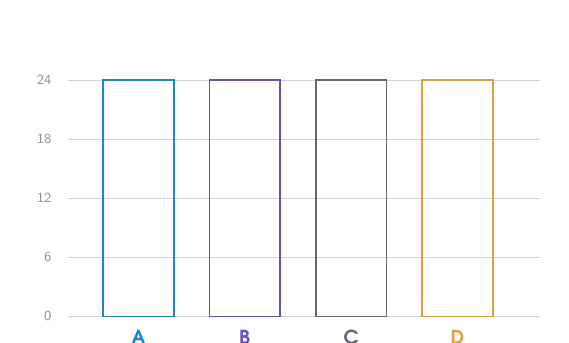
\begin{tikzpicture}[x=1mm,y=1mm,font=\uifont\tiny]
\foreach \v in {0,6,12,18,24}{\draw[line!80,line width=0.3pt] (0,\v*1.25) -- (60,\v*1.25); \node[anchor=east,text=mute] at (-0.8,\v*1.25) {\v};}
\foreach \b/\c [count=\i] in {A/accent,B/mJJK,C/ink!70,D/vault}{
  \draw[\c,line width=0.6pt] (\i*13.5-9,0) rectangle (\i*13.5+0,30);
  \node[text=\c,font=\hfont\bfseries\scriptsize] at (\i*13.5-4.5,-2.6) {\b};}
\end{tikzpicture}
\end{minipage}

% ---------------------------------------------------------------- Ex 2
\newcommand{\dq}[5]{% #1 num, #2 word, #3 a, #4 b, #5 c
  \begin{minipage}[t]{\linewidth}\RaggedRight
  \num{#1}\enspace\word{#2}\par\vspace{0.5mm}
  {\small\begin{tabular}{@{}l@{\ }p{0.88\linewidth}@{}}
  {\uifont\bfseries\scriptsize\color{mute}a} & #3\\
  {\uifont\bfseries\scriptsize\color{mute}b} & #4\\
  {\uifont\bfseries\scriptsize\color{mute}c} & #5\\
  \end{tabular}}\par
  {\scriptsize\color{mute}decoys:}\ \blank[2.2cm]\ {\scriptsize\color{mute}/}\ \blank[2.2cm]
  \end{minipage}\par\vspace{3.2mm}}

\exhead{2}{Decoys}{\tgL{M}{meaning}\,\tgL{N}{nuance}}{\mThink\,\mTimed}
\instr{Circle the correct definition. Careful: the two wrong options are not random — each one is the definition of \emph{another word in your vault}. Bonus point for every decoy you can name. Aim for under six minutes.}
\begin{multicols}{2}
\dq{1}{latent}{about to happen very soon}{present from birth, not learned}{existing, but not yet developed, active or visible}
\dq{2}{leniency}{a lack of care and attention}{the quality of being less strict than expected when punishing}{a feeling of strong dislike}
\dq{3}{plight}{a serious public promise}{an urgent, emotional request}{a difficult or dangerous situation}
\dq{4}{forfeit}{to lose or give something up as a penalty}{to refuse to give something that is wanted}{to make secret information known}
\dq{5}{discretion}{care not to embarrass anyone or reveal private things}{close and careful examination}{praise that is too much, or not sincere}
\dq{6}{linger}{to walk slowly and casually, for pleasure}{to stay longer than necessary; to continue to exist}{to worry about something}
\dq{7}{dwindle}{to fall suddenly from a high level}{to become worse in quality or behaviour}{to become gradually smaller or fewer}
\dq{8}{engulf}{to surround or cover something completely}{to trap someone, as if in a net}{to destroy completely}
\dq{9}{gullible}{not aware of what is happening around you}{easily tricked or deceived}{not easily convinced; full of doubt}
\dq{10}{bleak}{(of land) too poor for plants to grow}{sad and quiet, with no energy}{cold and empty; offering little hope}
\dq{11}{devious}{rude and showing no respect}{dishonest in a clever, indirect way}{wicked or criminal in nature}
\dq{12}{meagre}{small in amount and not enough}{small and weak (of a person)}{enough, or more than enough}
\end{multicols}

% ---------------------------------------------------------------- Ex 3
\exhead[112mm]{3}{Here goes nothing}{\tgL{M}{meaning}\,\tgL{F}{spelling}}{\mThink}
\instr{Solve the clues and write one letter per box. The shaded first column hides a phrase from your vault — if it reads like nonsense, one of your answers is wrong. That is the self-check.}
\noindent\begin{minipage}[t]{0.37\linewidth}\vspace{0pt}
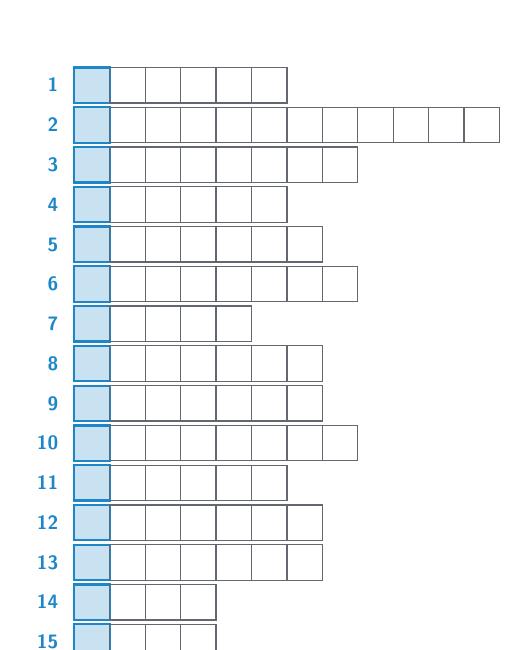
\begin{tikzpicture}[x=1mm,y=-1mm]
\node[anchor=east,font=\uifont\bfseries\scriptsize,text=accent] at (4.2,2.25) {1};
\fill[accent!24] (5.00,0.00) rectangle +(4.5,4.5);
\draw[accent,line width=0.8pt] (5.00,0.00) rectangle +(4.5,4.5);
\draw[ink!70,line width=0.45pt] (9.50,0.00) rectangle +(4.5,4.5);
\draw[ink!70,line width=0.45pt] (14.00,0.00) rectangle +(4.5,4.5);
\draw[ink!70,line width=0.45pt] (18.50,0.00) rectangle +(4.5,4.5);
\draw[ink!70,line width=0.45pt] (23.00,0.00) rectangle +(4.5,4.5);
\draw[ink!70,line width=0.45pt] (27.50,0.00) rectangle +(4.5,4.5);
\node[anchor=east,font=\uifont\bfseries\scriptsize,text=accent] at (4.2,7.30) {2};
\fill[accent!24] (5.00,5.05) rectangle +(4.5,4.5);
\draw[accent,line width=0.8pt] (5.00,5.05) rectangle +(4.5,4.5);
\draw[ink!70,line width=0.45pt] (9.50,5.05) rectangle +(4.5,4.5);
\draw[ink!70,line width=0.45pt] (14.00,5.05) rectangle +(4.5,4.5);
\draw[ink!70,line width=0.45pt] (18.50,5.05) rectangle +(4.5,4.5);
\draw[ink!70,line width=0.45pt] (23.00,5.05) rectangle +(4.5,4.5);
\draw[ink!70,line width=0.45pt] (27.50,5.05) rectangle +(4.5,4.5);
\draw[ink!70,line width=0.45pt] (32.00,5.05) rectangle +(4.5,4.5);
\draw[ink!70,line width=0.45pt] (36.50,5.05) rectangle +(4.5,4.5);
\draw[ink!70,line width=0.45pt] (41.00,5.05) rectangle +(4.5,4.5);
\draw[ink!70,line width=0.45pt] (45.50,5.05) rectangle +(4.5,4.5);
\draw[ink!70,line width=0.45pt] (50.00,5.05) rectangle +(4.5,4.5);
\draw[ink!70,line width=0.45pt] (54.50,5.05) rectangle +(4.5,4.5);
\node[anchor=east,font=\uifont\bfseries\scriptsize,text=accent] at (4.2,12.35) {3};
\fill[accent!24] (5.00,10.10) rectangle +(4.5,4.5);
\draw[accent,line width=0.8pt] (5.00,10.10) rectangle +(4.5,4.5);
\draw[ink!70,line width=0.45pt] (9.50,10.10) rectangle +(4.5,4.5);
\draw[ink!70,line width=0.45pt] (14.00,10.10) rectangle +(4.5,4.5);
\draw[ink!70,line width=0.45pt] (18.50,10.10) rectangle +(4.5,4.5);
\draw[ink!70,line width=0.45pt] (23.00,10.10) rectangle +(4.5,4.5);
\draw[ink!70,line width=0.45pt] (27.50,10.10) rectangle +(4.5,4.5);
\draw[ink!70,line width=0.45pt] (32.00,10.10) rectangle +(4.5,4.5);
\draw[ink!70,line width=0.45pt] (36.50,10.10) rectangle +(4.5,4.5);
\node[anchor=east,font=\uifont\bfseries\scriptsize,text=accent] at (4.2,17.40) {4};
\fill[accent!24] (5.00,15.15) rectangle +(4.5,4.5);
\draw[accent,line width=0.8pt] (5.00,15.15) rectangle +(4.5,4.5);
\draw[ink!70,line width=0.45pt] (9.50,15.15) rectangle +(4.5,4.5);
\draw[ink!70,line width=0.45pt] (14.00,15.15) rectangle +(4.5,4.5);
\draw[ink!70,line width=0.45pt] (18.50,15.15) rectangle +(4.5,4.5);
\draw[ink!70,line width=0.45pt] (23.00,15.15) rectangle +(4.5,4.5);
\draw[ink!70,line width=0.45pt] (27.50,15.15) rectangle +(4.5,4.5);
\node[anchor=east,font=\uifont\bfseries\scriptsize,text=accent] at (4.2,22.45) {5};
\fill[accent!24] (5.00,20.20) rectangle +(4.5,4.5);
\draw[accent,line width=0.8pt] (5.00,20.20) rectangle +(4.5,4.5);
\draw[ink!70,line width=0.45pt] (9.50,20.20) rectangle +(4.5,4.5);
\draw[ink!70,line width=0.45pt] (14.00,20.20) rectangle +(4.5,4.5);
\draw[ink!70,line width=0.45pt] (18.50,20.20) rectangle +(4.5,4.5);
\draw[ink!70,line width=0.45pt] (23.00,20.20) rectangle +(4.5,4.5);
\draw[ink!70,line width=0.45pt] (27.50,20.20) rectangle +(4.5,4.5);
\draw[ink!70,line width=0.45pt] (32.00,20.20) rectangle +(4.5,4.5);
\node[anchor=east,font=\uifont\bfseries\scriptsize,text=accent] at (4.2,27.50) {6};
\fill[accent!24] (5.00,25.25) rectangle +(4.5,4.5);
\draw[accent,line width=0.8pt] (5.00,25.25) rectangle +(4.5,4.5);
\draw[ink!70,line width=0.45pt] (9.50,25.25) rectangle +(4.5,4.5);
\draw[ink!70,line width=0.45pt] (14.00,25.25) rectangle +(4.5,4.5);
\draw[ink!70,line width=0.45pt] (18.50,25.25) rectangle +(4.5,4.5);
\draw[ink!70,line width=0.45pt] (23.00,25.25) rectangle +(4.5,4.5);
\draw[ink!70,line width=0.45pt] (27.50,25.25) rectangle +(4.5,4.5);
\draw[ink!70,line width=0.45pt] (32.00,25.25) rectangle +(4.5,4.5);
\draw[ink!70,line width=0.45pt] (36.50,25.25) rectangle +(4.5,4.5);
\node[anchor=east,font=\uifont\bfseries\scriptsize,text=accent] at (4.2,32.55) {7};
\fill[accent!24] (5.00,30.30) rectangle +(4.5,4.5);
\draw[accent,line width=0.8pt] (5.00,30.30) rectangle +(4.5,4.5);
\draw[ink!70,line width=0.45pt] (9.50,30.30) rectangle +(4.5,4.5);
\draw[ink!70,line width=0.45pt] (14.00,30.30) rectangle +(4.5,4.5);
\draw[ink!70,line width=0.45pt] (18.50,30.30) rectangle +(4.5,4.5);
\draw[ink!70,line width=0.45pt] (23.00,30.30) rectangle +(4.5,4.5);
\node[anchor=east,font=\uifont\bfseries\scriptsize,text=accent] at (4.2,37.60) {8};
\fill[accent!24] (5.00,35.35) rectangle +(4.5,4.5);
\draw[accent,line width=0.8pt] (5.00,35.35) rectangle +(4.5,4.5);
\draw[ink!70,line width=0.45pt] (9.50,35.35) rectangle +(4.5,4.5);
\draw[ink!70,line width=0.45pt] (14.00,35.35) rectangle +(4.5,4.5);
\draw[ink!70,line width=0.45pt] (18.50,35.35) rectangle +(4.5,4.5);
\draw[ink!70,line width=0.45pt] (23.00,35.35) rectangle +(4.5,4.5);
\draw[ink!70,line width=0.45pt] (27.50,35.35) rectangle +(4.5,4.5);
\draw[ink!70,line width=0.45pt] (32.00,35.35) rectangle +(4.5,4.5);
\node[anchor=east,font=\uifont\bfseries\scriptsize,text=accent] at (4.2,42.65) {9};
\fill[accent!24] (5.00,40.40) rectangle +(4.5,4.5);
\draw[accent,line width=0.8pt] (5.00,40.40) rectangle +(4.5,4.5);
\draw[ink!70,line width=0.45pt] (9.50,40.40) rectangle +(4.5,4.5);
\draw[ink!70,line width=0.45pt] (14.00,40.40) rectangle +(4.5,4.5);
\draw[ink!70,line width=0.45pt] (18.50,40.40) rectangle +(4.5,4.5);
\draw[ink!70,line width=0.45pt] (23.00,40.40) rectangle +(4.5,4.5);
\draw[ink!70,line width=0.45pt] (27.50,40.40) rectangle +(4.5,4.5);
\draw[ink!70,line width=0.45pt] (32.00,40.40) rectangle +(4.5,4.5);
\node[anchor=east,font=\uifont\bfseries\scriptsize,text=accent] at (4.2,47.70) {10};
\fill[accent!24] (5.00,45.45) rectangle +(4.5,4.5);
\draw[accent,line width=0.8pt] (5.00,45.45) rectangle +(4.5,4.5);
\draw[ink!70,line width=0.45pt] (9.50,45.45) rectangle +(4.5,4.5);
\draw[ink!70,line width=0.45pt] (14.00,45.45) rectangle +(4.5,4.5);
\draw[ink!70,line width=0.45pt] (18.50,45.45) rectangle +(4.5,4.5);
\draw[ink!70,line width=0.45pt] (23.00,45.45) rectangle +(4.5,4.5);
\draw[ink!70,line width=0.45pt] (27.50,45.45) rectangle +(4.5,4.5);
\draw[ink!70,line width=0.45pt] (32.00,45.45) rectangle +(4.5,4.5);
\draw[ink!70,line width=0.45pt] (36.50,45.45) rectangle +(4.5,4.5);
\node[anchor=east,font=\uifont\bfseries\scriptsize,text=accent] at (4.2,52.75) {11};
\fill[accent!24] (5.00,50.50) rectangle +(4.5,4.5);
\draw[accent,line width=0.8pt] (5.00,50.50) rectangle +(4.5,4.5);
\draw[ink!70,line width=0.45pt] (9.50,50.50) rectangle +(4.5,4.5);
\draw[ink!70,line width=0.45pt] (14.00,50.50) rectangle +(4.5,4.5);
\draw[ink!70,line width=0.45pt] (18.50,50.50) rectangle +(4.5,4.5);
\draw[ink!70,line width=0.45pt] (23.00,50.50) rectangle +(4.5,4.5);
\draw[ink!70,line width=0.45pt] (27.50,50.50) rectangle +(4.5,4.5);
\node[anchor=east,font=\uifont\bfseries\scriptsize,text=accent] at (4.2,57.80) {12};
\fill[accent!24] (5.00,55.55) rectangle +(4.5,4.5);
\draw[accent,line width=0.8pt] (5.00,55.55) rectangle +(4.5,4.5);
\draw[ink!70,line width=0.45pt] (9.50,55.55) rectangle +(4.5,4.5);
\draw[ink!70,line width=0.45pt] (14.00,55.55) rectangle +(4.5,4.5);
\draw[ink!70,line width=0.45pt] (18.50,55.55) rectangle +(4.5,4.5);
\draw[ink!70,line width=0.45pt] (23.00,55.55) rectangle +(4.5,4.5);
\draw[ink!70,line width=0.45pt] (27.50,55.55) rectangle +(4.5,4.5);
\draw[ink!70,line width=0.45pt] (32.00,55.55) rectangle +(4.5,4.5);
\node[anchor=east,font=\uifont\bfseries\scriptsize,text=accent] at (4.2,62.85) {13};
\fill[accent!24] (5.00,60.60) rectangle +(4.5,4.5);
\draw[accent,line width=0.8pt] (5.00,60.60) rectangle +(4.5,4.5);
\draw[ink!70,line width=0.45pt] (9.50,60.60) rectangle +(4.5,4.5);
\draw[ink!70,line width=0.45pt] (14.00,60.60) rectangle +(4.5,4.5);
\draw[ink!70,line width=0.45pt] (18.50,60.60) rectangle +(4.5,4.5);
\draw[ink!70,line width=0.45pt] (23.00,60.60) rectangle +(4.5,4.5);
\draw[ink!70,line width=0.45pt] (27.50,60.60) rectangle +(4.5,4.5);
\draw[ink!70,line width=0.45pt] (32.00,60.60) rectangle +(4.5,4.5);
\node[anchor=east,font=\uifont\bfseries\scriptsize,text=accent] at (4.2,67.90) {14};
\fill[accent!24] (5.00,65.65) rectangle +(4.5,4.5);
\draw[accent,line width=0.8pt] (5.00,65.65) rectangle +(4.5,4.5);
\draw[ink!70,line width=0.45pt] (9.50,65.65) rectangle +(4.5,4.5);
\draw[ink!70,line width=0.45pt] (14.00,65.65) rectangle +(4.5,4.5);
\draw[ink!70,line width=0.45pt] (18.50,65.65) rectangle +(4.5,4.5);
\node[anchor=east,font=\uifont\bfseries\scriptsize,text=accent] at (4.2,72.95) {15};
\fill[accent!24] (5.00,70.70) rectangle +(4.5,4.5);
\draw[accent,line width=0.8pt] (5.00,70.70) rectangle +(4.5,4.5);
\draw[ink!70,line width=0.45pt] (9.50,70.70) rectangle +(4.5,4.5);
\draw[ink!70,line width=0.45pt] (14.00,70.70) rectangle +(4.5,4.5);
\draw[ink!70,line width=0.45pt] (18.50,70.70) rectangle +(4.5,4.5);
\end{tikzpicture}
\end{minipage}\hfill
\begin{minipage}[t]{0.6\linewidth}\vspace{0pt}\small\RaggedRight
\setlength{\parskip}{2.1pt}
\num{1} A person who lives alone and avoids other people. \emph{After exam week I turn into a total} \dots\par
\num{2} Making you feel extremely happy and full of energy: \emph{an \dots{} final lap.}\par
\num{3} Famous and respected for something: \emph{Leuven is \dots{} for its university and its beer.}\par
\num{4} To treat two things as the same: \emph{Don’t \dots{} being busy with being productive.}\par
\num{5} A quick, incomplete view: \emph{I caught a \dots{} of the exam paper on the desk.}\par
\num{6} To fail to notice: \emph{It’s easy to \dots{} a minus sign in a long derivation.}\par
\num{7} To force a tenant to leave a property, usually by law.\par
\num{8} Having far too much work: \emph{I’m \dots{} this week — three deadlines.}\par
\num{9} To fail to look after something: \emph{Don’t \dots{} your sleep in exam season.}\par
\num{10} Complete; or openly and directly: \emph{an \dots{} lie} \mdot{} \emph{she refused \dots}\par
\num{11} To make small repairs or changes, often as an amateur: \emph{he loves to \dots{} with old PCs.}\par
\num{12} A small number — or a person who is hard to control: \emph{Only a \dots{} came.} \mdot{} \emph{That puppy is a real \dots}\par
\num{13} \emph{To be \dots{} to do something} = to want to do it very much, very soon.\par
\num{14} Too interested in other people’s private lives.\par
\num{15} Courage and determination to keep going when things get hard.\par
\end{minipage}
\par\vspace{2.5mm}
\noindent{\small\textbf{The hidden phrase:}}\enspace\blank[5.5cm]\enspace{\small When would you say it?}\enspace\wfill

% =====================================================================
% PART 2 — GRASP
% =====================================================================
\partbanner{PART 2}{GRASP}{Get a grip on the meaning — and then on the other meanings. Plus spelling and sound.}

% ---------------------------------------------------------------- Ex 4
\newcommand{\owt}[4]{% #1 num, #2 a, #3 b, #4 c
  \needsp{17mm}\noindent\begin{minipage}[c]{0.79\linewidth}\RaggedRight\small
  \makebox[5mm][l]{\num{#1}}{\uifont\bfseries\scriptsize\color{mute}a}\enspace #2\par
  \hspace*{5mm}{\uifont\bfseries\scriptsize\color{mute}b}\enspace #3\par
  \hspace*{5mm}{\uifont\bfseries\scriptsize\color{mute}c}\enspace #4
  \end{minipage}\hfill
  \begin{minipage}[c]{0.19\linewidth}\raggedleft\tikz[baseline]{\draw[accent,line width=0.7pt,rounded corners=1mm] (0,0) rectangle (30mm,7.5mm);}\end{minipage}
  \par\vspace{2.6mm}}
\newcommand{\bl}{\blank[1.7cm]}

\exhead{4}{One word, three jobs}{\tgL{S}{senses}\,\tgL{C}{collocation}}{\mWrite\,\mThink}
\instr{One word from your vault fits all three gaps — in three different senses. Write it once, in the box. The gaps may need a different form (\emph{-s, -ed, -ing}). Most of these senses are on your cards; a few are the ones your cards forgot.}
\vspace{1mm}
\owt{1}{I’ve never been very \bl{} on horror films, to be honest.}{You need a \bl{} eye to spot a typo in a 40-page lab report.}{Careful — the new kitchen knife has a really \bl{} edge.}
\owt{2}{We spent Sunday on the Belgian \bl, eating waffles in the wind.}{He \bl{} through first year without opening a single book.}{The bike \bl{} down the hill while I took my feet off the pedals.}
\owt{3}{Our kot is on the top \bl{} — and there’s no lift, of course.}{Her question completely \bl{} me; I had no idea what to say.}{After the talk, the chair gave the \bl{} to the audience for questions.}
\owt{4}{We won by \bl{} luck — their best player had food poisoning.}{The coastal path ends at a \bl{} drop into the sea.}{She wore a \bl, almost see-through blouse over a black top.}
\owt{5}{The death \bl{} from the floods has risen to thirty.}{On most French motorways you have to pay a \bl.}{Somewhere in the old town, a church bell began to \bl.}
\owt{6}{Most arguments in our house \bl{} from one thing: the washing-up.}{The new rules are meant to \bl{} the flow of fake news.}{Cut each flower’s \bl{} at an angle before you put it in water.}
\owt{7}{There’s been a \bl{} in demand for student rooms this year.}{I felt a \bl{} of panic when I turned over the exam paper.}{A power \bl{} fried my PC’s motherboard during the storm.}
\owt{8}{The firefighter who saved the kitten was \bl{} as a hero.}{Raise your arm to \bl{} a taxi.}{Lumps of \bl{} the size of marbles dented every car in the street.}
\owt{9}{A fish bone got \bl{} in his throat.}{We decided to \bl{} a formal complaint with the university.}{For the ski trip we rented a wooden \bl{} in the Alps.}
\owt{10}{The deadline is putting a lot of \bl{} on the whole team.}{I \bl{} a muscle in my calf on my long run.}{\bl{} the pasta, but keep a cup of the cooking water.}

% ---------------------------------------------------------------- Ex 5
\newcommand{\knob}[4]{% #1 title, #2 question, #3 scrambled words, #4 number of slots
  \begin{minipage}[t]{\linewidth}
  {\hfont\bfseries\small\color{ink}#1}\enspace{\small\color{inksoft}#2}\par\vspace{0.6mm}
  {\small\uifont\color{accentdark}#3}\par\vspace{1.6mm}
  \begin{tikzpicture}[x=1mm,y=1mm]
  \shade[left color=accent!6,right color=accent,rounded corners=1.2mm] (0,0) rectangle (82,2.4);
  \pgfmathsetmacro\stepw{82/#4}
  \foreach \i in {1,...,#4}{
    \pgfmathsetmacro\cx{(\i-0.5)*\stepw}
    \fill[white] (\cx,1.2) circle (0.95); \draw[ink,line width=0.45pt] (\cx,1.2) circle (0.95);
    \draw[line,line width=0.5pt] (\cx-\stepw/2+1.6,-5.2) -- (\cx+\stepw/2-1.6,-5.2);
  }
  \node[anchor=south west,font=\uifont\tiny,text=mute,inner sep=0pt] at (0,3.2) {weakest};
  \node[anchor=south east,font=\uifont\tiny,text=mute,inner sep=0pt] at (82,3.2) {strongest};
  \end{tikzpicture}
  \end{minipage}}

\exhead{5}{Volume knobs}{\tgL{N}{nuance}}{\mThink}
\instr{Each knob turns one idea up from weakest to strongest. Put the words in order on the lines. Near-synonyms are where meaning gets fuzzy after a break — this is how you sharpen it.}
\vspace{1mm}
\noindent\begin{minipage}[t]{0.48\linewidth}
\knob{EFFORT}{How hard are you working?}{coast \enspace\mdot\enspace slack off \enspace\mdot\enspace work your tail off \enspace\mdot\enspace buckle down}{4}
\par\vspace{5mm}
\knob{TROUBLE}{How bad is it?}{calamity \enspace\mdot\enspace snag \enspace\mdot\enspace ordeal}{3}
\par\vspace{5mm}
\knob{LAUGHTER}{How loud is it?}{crack up \enspace\mdot\enspace grin \enspace\mdot\enspace giggle}{3}
\end{minipage}\hfill
\begin{minipage}[t]{0.48\linewidth}
\knob{RESISTANCE}{How firmly are you saying no?}{reluctant \enspace\mdot\enspace defiant \enspace\mdot\enspace hesitant \enspace\mdot\enspace balk at}{4}
\par\vspace{5mm}
\knob{CONFLICT}{How violent is it?}{onslaught \enspace\mdot\enspace bickering \enspace\mdot\enspace quarrel}{3}
\par\vspace{5mm}
\knob{NERVE}{How shameless is it?}{brazen \enspace\mdot\enspace sassy \enspace\mdot\enspace impudent}{3}
\end{minipage}
\par\vspace{4mm}\needsp{24mm}
\noindent{\small\textbf{Turn it up.} Write one sentence about your last week using the \emph{strongest} word from any two knobs.}
\wlines{2}

% ---------------------------------------------------------------- Ex 6
\newcommand{\chipw}[1]{\tikz[baseline=(c.base)]{\node[inner xsep=3pt,inner ysep=2.2pt,draw=line,rounded corners=1.5pt,font=\uifont\large](c){#1};}}
\exhead{6}{Mic check}{\tgL{F}{spelling \& sound}\,\tgL{B}{British}}{\mSpeak\,\mThink\,\UK}
\instr{Half of understanding British players on voice chat is knowing how words \emph{sound}; half of writing well is knowing how they are \emph{spelt}. Four quick checks.}

\noindent{\hfont\bfseries\small\color{accent}A}\enspace{\small\textbf{Spellcheck can’t save you.} Each sentence has one wrong word that \emph{sounds} right. Write the correct word.}\par\vspace{1mm}
\begin{multicols}{2}\small\RaggedRight
\num{1} I’ve been working my tale off for this exam. \enspace\blank[1.4cm]\par\vspace{1.2mm}
\num{2} The bus fair to Heverlee went up again. \enspace\blank[1.4cm]\par\vspace{1.2mm}
\num{3} Running a half-marathon in under two hours is quite a feet. \enspace\blank[1.4cm]\par\vspace{1.2mm}
\num{4} Stop medalling in my love life! \enspace\blank[1.4cm]\par\vspace{1.2mm}
\num{5} The bins reak in this heat. \enspace\blank[1.4cm]\par\vspace{1.2mm}
\num{6} My soul reason for joining was the free pizza. \enspace\blank[1.4cm]\par\vspace{1.2mm}
\num{7} Add two cups of flower and a pinch of salt. \enspace\blank[1.4cm]\par\vspace{1.2mm}
\num{8} I booked a long-hall flight to São Paulo. \enspace\blank[1.4cm]\par
\end{multicols}
\vspace{1.5mm}
\noindent{\hfont\bfseries\small\color{accent}B}\enspace{\small\textbf{Silent letters.} Circle every letter you do \emph{not} pronounce.}\par\vspace{1.6mm}
\noindent\hfill\chipw{subtle}\hfill\chipw{heirloom}\hfill\chipw{numb}\hfill\chipw{knack}\hfill\chipw{wrestling}\hfill\par\vspace{1.6mm}
\noindent\hfill\chipw{wrath}\hfill\chipw{reigning}\hfill\chipw{psyche}\hfill\chipw{doughy}\hfill\chipw{listen up}\hfill\par
\vspace{2.5mm}
\noindent{\hfont\bfseries\small\color{accent}C}\enspace{\small\textbf{The British {\normalfont\textipa{/A:/}}.} In standard southern British English, \emph{some} words with the letter \emph{a} take the long vowel of \emph{car}, where Americans say the short vowel of \emph{cat}. Tick the six that do.}\par\vspace{1.4mm}
{\small\uifont\noindent\begin{tabular*}{\linewidth}{@{\extracolsep{\fill}}llllll@{}}
\cbox\ grasp & \cbox\ ample & \cbox\ chant & \cbox\ anvil & \cbox\ slander & \cbox\ dashing\\[1.4mm]
\cbox\ scram & \cbox\ rascal & \cbox\ racket & \cbox\ half-pint & \cbox\ tandem & \cbox\ laughingstock\\
\end{tabular*}}
\par\vspace{2.5mm}
\noindent{\hfont\bfseries\small\color{accent}D}\enspace{\small\textbf{Stress.} Underline the stressed syllable.}\par\vspace{1.4mm}
{\uifont\noindent\begin{tabular*}{\linewidth}{@{\extracolsep{\fill}}lllll@{}}
un·pre·ce·den·ted & om·ni·scient & ex·em·pla·ry & ca·la·mi·ty & sab·ba·ti·cal\\[1.4mm]
con·tin·gen·cy & bu·reau·crat & vo·ci·fer·ous·ly & con·vo·lu·ted & le·ni·en·cy\\
\end{tabular*}}
\par\vspace{2mm}
\begin{speakbox}
\mSpeak\enspace\textbf{Say it, then check it.} Read Part D aloud three times and record yourself. Then play the UK audio for each word on the Cambridge Dictionary website and compare. One word you got wrong = one note on that card in your vault.
\end{speakbox}

% =====================================================================
% PART 3 — FINESSE
% =====================================================================
\partbanner{PART 3}{FINESSE}{Delicate skill (your MHA card). Same family, different jobs: connotation, near-synonyms and the company words keep.}

% ---------------------------------------------------------------- Ex 7
\newcommand{\ci}[1]{\lbox{4.2mm}\enspace{\uifont #1}}
\exhead{7}{Compliment or insult?}{\tgL{N}{connotation}\,\tgL{R}{register}}{\mThink}
\instr{Someone at your student job — or in your Discord server — describes you with one of these words. Is it a \textbf{C}ompliment, an \textbf{I}nsult, or does it \textbf{D}epend (on context, tone, or which side of the Atlantic you are on)? Write C, I or D in the box.}
\vspace{1mm}
{\small\noindent\begin{tabular*}{\linewidth}{@{\extracolsep{\fill}}llll@{}}
\ci{shrewd} & \ci{gullible} & \ci{resourceful} & \ci{stuck-up}\\[2.4mm]
\ci{nimble} & \ci{cunning} & \ci{nosy} & \ci{exemplary}\\[2.4mm]
\ci{scrappy} & \ci{cocky} & \ci{feisty} & \ci{naive}\\[2.4mm]
\ci{smooth-talking} & \ci{laid-back} & \ci{pigheaded} & \ci{defiant}\\[2.4mm]
\ci{dashing} & \ci{obnoxious} & \ci{mischievous} & \ci{portly}\\
\end{tabular*}}
\par\vspace{3mm}
\noindent{\small\textbf{Flip it.} Choose one of your D words. Write a sentence where it is praise and one where it stings.}
\wlines{2}

% ---------------------------------------------------------------- Ex 8
\newcommand{\fh}[1]{{\uifont\bfseries\footnotesize\color{accent}#1}}
\newcommand{\fr}[1]{{\uifont\bfseries\small #1} & \cbox & \cbox & \cbox & \cbox & \cbox & \cbox\\[0.6mm]}
\exhead{8}{Not quite twins}{\tgL{N}{near-synonyms}\,\tgL{C}{collocation}}{\mThink\,\mWrite}
\instr{Near-synonyms are your vault’s most dangerous neighbours. Map what makes each one different, then use the map.}

\noindent{\hfont\bfseries\small\color{accent}A}\enspace{\small\textbf{Stopping things.} Tick \emph{every} feature that applies.}\par\vspace{1.2mm}
\noindent\begin{minipage}[c]{0.43\linewidth}
{\renewcommand{\arraystretch}{1.12}\begin{tabular}{@{}l@{\hspace{3mm}}c@{\hspace{2.2mm}}c@{\hspace{2.2mm}}c@{\hspace{2.2mm}}c@{\hspace{2.2mm}}c@{\hspace{2.2mm}}c@{}}
 & \fh{\ding{172}} & \fh{\ding{173}} & \fh{\ding{174}} & \fh{\ding{175}} & \fh{\ding{176}} & \fh{\ding{177}}\\
\fr{hinder}\fr{impede}\fr{thwart}\fr{foil}\fr{ward off}\fr{fend off}\fr{hold off}
\end{tabular}}
\end{minipage}\hfill
\begin{minipage}[c]{0.54\linewidth}\small\RaggedRight
\fh{\ding{172}} slows it down or makes it harder (it may still happen)\par
\fh{\ding{173}} stops a plan, plot or attempt completely\par
\fh{\ding{174}} keeps a danger, an illness or an attacker away\par
\fh{\ding{175}} also works with difficult questions or criticism\par
\fh{\ding{176}} can also mean \emph{wait before doing something}\par
\fh{\ding{177}} formal — at home in reports and essays
\end{minipage}
\par\vspace{2mm}
{\small\begin{multicols}{2}\RaggedRight
\num{a} Police \blank[1.8cm] a plot to steal paintings from the museum.\par\vspace{1.3mm}
\num{b} Garlic was once believed to \blank[1.8cm] evil spirits.\par\vspace{1.3mm}
\num{c} Heavy snow \blank[1.8cm] the rescue effort for two days.\par\vspace{1.3mm}
\num{d} The minister \blank[1.8cm] awkward questions about the budget.\par\vspace{1.3mm}
\num{e} Let’s \blank[1.8cm] booking the flights until the prices drop.\par\vspace{1.3mm}
\num{f} \emph{(lab report)} Insufficient lighting may \blank[1.8cm] the operator’s concentration.\par
\end{multicols}}
\needsp{62mm}\vspace{1.5mm}
\noindent{\hfont\bfseries\small\color{accent}B}\enspace{\small\textbf{Who works for whom?} Tick the \emph{one} feature that defines each word best.}\par\vspace{1.2mm}
\noindent\begin{minipage}[c]{0.43\linewidth}
{\renewcommand{\arraystretch}{1.12}\begin{tabular}{@{}l@{\hspace{3mm}}c@{\hspace{2.2mm}}c@{\hspace{2.2mm}}c@{\hspace{2.2mm}}c@{\hspace{2.2mm}}c@{\hspace{2.2mm}}c@{}}
 & \fh{\ding{172}} & \fh{\ding{173}} & \fh{\ding{174}} & \fh{\ding{175}} & \fh{\ding{176}} & \fh{\ding{177}}\\
\fr{henchman}\fr{sidekick}\fr{crony}\fr{lackey}\fr{underling}\fr{pawn}
\end{tabular}}
\end{minipage}\hfill
\begin{minipage}[c]{0.54\linewidth}\small\RaggedRight
\fh{\ding{172}} does the dirty work for a villain or a crime boss\par
\fh{\ding{173}} a loyal companion — often the funny one\par
\fh{\ding{174}} a friend who gets unfair favours (politics, business)\par
\fh{\ding{175}} servile: will do anything they are told\par
\fh{\ding{176}} simply lower in rank — said with contempt\par
\fh{\ding{177}} used or manipulated by someone more powerful
\end{minipage}
\par\vspace{2mm}
{\small\begin{multicols}{2}\RaggedRight
\num{g} The president gave all the top jobs to his \blank[1.8cm].\par\vspace{1.3mm}
\num{h} Every superhero needs a wisecracking \blank[1.8cm].\par\vspace{1.3mm}
\num{i} The villain sent two \blank[1.8cm] to break into the lab.\par\vspace{1.3mm}
\num{j} I’m nobody’s \blank[1.8cm] — fetch your own coffee.\par\vspace{1.3mm}
\num{k} She realised she had been a \blank[1.8cm] in their game all along.\par\vspace{1.3mm}
\num{l} Our manager never talks to his \blank[1.8cm]; he just sends emails.\par
\end{multicols}}
\needsp{40mm}\vspace{1.5mm}
\noindent{\hfont\bfseries\small\color{accent}C}\enspace{\small\textbf{Pick the precise one.}}\par\vspace{1mm}
{\small\begin{multicols}{2}\RaggedRight
\num{m} Babies have an \opt{innate}{inherent} ability to recognise faces.\par\vspace{1.1mm}
\num{n} Every investment carries an \opt{innate}{inherent} risk.\par\vspace{1.1mm}
\num{o} I \optt{seldom}{scarcely}{merely} go out on weeknights.\par\vspace{1.1mm}
\num{p} I could \optt{seldom}{scarcely}{merely} hear him over the music.\par\vspace{1.1mm}
\num{q} It’s \optt{seldom}{scarcely}{merely} a scratch — stop fussing.\par\vspace{1.1mm}
\num{r} This is a matter of the \opt{utmost}{upmost} importance.\par\vspace{1.1mm}
\num{s} Can you \opt{assure}{ensure} that the lab is locked tonight?\par\vspace{1.1mm}
\num{t} Police are still trying to establish the suspect’s \opt{whereabouts}{venue}.\par
\end{multicols}}

% ---------------------------------------------------------------- Ex 9
\newcommand{\fork}[5]{% #1 verb, #2-#5 nouns
  \begin{tcolorbox}[enhanced,colback=white,colframe=line,boxrule=0.5pt,arc=1.5mm,left=2mm,right=2mm,top=1mm,bottom=1.2mm,
     title={\hfont\bfseries\small\MakeUppercase{#1}},coltitle=white,colbacktitle=accent,toptitle=0.4mm,bottomtitle=0.4mm,fontupper=\small\uifont]
  #2\par #3\par #4\par #5\par\vspace{1mm}
  {\color{mute}\scriptsize odd one goes with:}\ \blank[1.5cm]
  \end{tcolorbox}}
\exhead[120mm]{9}{The odd one out}{\tgL{C}{collocation}}{\mThink}
\instr{Three of the nouns are natural partners of the verb; one is not. Cross out the intruder, then write the verb it \emph{does} go with. These pairs are exactly what turns a 7.5 into an 8 in writing.}
\vspace{1mm}
\noindent\begin{minipage}[t]{0.32\linewidth}
\fork{harbour}{a grudge}{doubts}{suspicions}{a threat}
\fork{evoke}{memories}{sympathy}{a response}{a decision}
\fork{wield}{power}{influence}{a sword}{an opinion}
\fork{strike}{a deal}{a balance}{a chord}{a conclusion}
\end{minipage}\hfill
\begin{minipage}[t]{0.32\linewidth}
\fork{impose}{a ban}{a curfew}{a fine}{a question}
\fork{forfeit}{the match}{a deposit}{a promise}{the right to appeal}
\fork{hone}{your skills}{a habit}{a technique}{your craft}
\fork{lodge}{a complaint}{an appeal}{a compliment}{an objection}
\end{minipage}\hfill
\begin{minipage}[t]{0.32\linewidth}
\fork{withhold}{information}{a meeting}{payment}{consent}
\fork{muster}{courage}{the strength}{attention}{support}
\fork{breach}{a contract}{a record}{security}{the rules}
\fork{tap into}{a market}{your potential}{a deadline}{a resource}
\end{minipage}

% =====================================================================
% PART 4 — CHIP AWAY
% =====================================================================
\partbanner{PART 4}{CHIP AWAY}{Phrasal verbs: small words doing big work. They come back the way you lost them — bit by bit.}

% ---------------------------------------------------------------- Ex 10
\newcommand{\atom}[4]{% #1 x (mm), #2 particle, #3 meaning, #4 rotation
  \draw[accent!45,line width=0.6pt,rotate around={#4:(#1,0)}] (#1,0) ellipse (12.5mm and 5mm);
  \fill[accent!45,rotate around={#4:(#1,0)}] ($(#1,0)+(12.5mm,0)$) circle (0.75mm);
  \fill[accent!45,rotate around={#4:(#1,0)}] ($(#1,0)+(-9mm,3.5mm)$) circle (0.75mm);
  \fill[accent] (#1,0) circle (6.4mm);
  \node[text=white,font=\hfont\bfseries\scriptsize,align=center] at (#1,0) {#2};
  \node[anchor=north,text=inksoft,font=\uifont\scriptsize,align=center,text width=27mm] at (#1,-8.5) {#3};}
\newcommand{\pv}[3]{\num{#1}\enspace{\uifont\bfseries #2}\enspace{\small\color{inksoft}— #3}\par\vspace{1.5mm}}
\newcommand{\pb}{\blank[0.95cm]}

\exhead[118mm]{10}{Particle physics}{\tgL{P}{phrasal verbs}}{\mThink\,\mWrite}
\instr{The little word after the verb is not random: each particle carries a core meaning. Use the map to guess the particle you have forgotten — you are an engineer, so treat it like physics.}
\begin{center}
\begin{tikzpicture}[x=1mm,y=1mm]
\atom{0}{OFF}{away from · disconnected · less}{18}
\atom{29}{UP}{completely · more · fixed}{-15}
\atom{58}{IN /\\INTO}{entering a room, a talk, a resource}{22}
\atom{87}{DOWN}{calmer · quieter · settled to work}{-20}
\atom{116}{AWAY /\\ALONG}{bit by bit · going with someone}{14}
\atom{145}{OUT\\OF}{leaving a state you were stuck in}{-12}
\end{tikzpicture}
\end{center}
\vspace{1mm}
\noindent{\hfont\bfseries\small\color{accent}A}\enspace{\small\textbf{Fill in the particle.}}\par\vspace{1.2mm}
\begin{multicols}{2}\small
\pv{1}{fend \pb}{keep an attacker or a question away}
\pv{2}{ward \pb}{keep an illness or danger away}
\pv{3}{brush \pb}{dismiss someone or an idea rudely}
\pv{4}{slack \pb}{work less hard than you should}
\pv{5}{drift \pb}{fall asleep slowly}
\pv{6}{pull \pb}{succeed at something difficult}
\pv{7}{patch \pb}{repair quickly; make friends again}
\pv{8}{stir \pb}{deliberately cause trouble}
\pv{9}{pile \pb}{accumulate}
\pv{10}{crack \pb}{burst out laughing}
\pv{11}{suck \pb{} to}{flatter someone to get an advantage}
\pv{12}{barge \pb}{enter rudely, without asking}
\pv{13}{butt \pb}{interrupt a conversation}
\pv{14}{step \pb}{get involved to help or to stop something}
\pv{15}{tap \pb}{access and use a resource}
\pv{16}{pipe \pb}{be quieter (not polite!)}
\pv{17}{buckle \pb}{start working seriously}
\pv{18}{chip \pb{} at}{reduce gradually, bit by bit}
\pv{19}{tag \pb}{go with someone, often uninvited}
\pv{20}{snap \pb{} of it}{stop feeling sorry for yourself}
\end{multicols}
\vspace{0.5mm}
\noindent{\hfont\bfseries\small\color{accent}B}\enspace{\small\textbf{Same family, different job.} Choose the right phrasal verb and put it in the right form.}\par\vspace{1.2mm}
{\small\begin{multicols}{2}\RaggedRight
\num{a} All those extra hours in the lab finally \blank[1.8cm]. \opt{pay off}{pull off}\par\vspace{1.3mm}
\num{b} Nobody thought we could win from 0--2 down, but we \blank[1.4cm] it \blank[0.9cm]! \opt{pay off}{pull off}\par\vspace{1.3mm}
\num{c} Sorry to \blank[1.6cm], but your laptop is on fire. \opt{barge in}{butt in}\par\vspace{1.3mm}
\num{d} He \blank[1.6cm] into my room without knocking. \opt{barge}{butt}\par\vspace{1.3mm}
\num{e} Vitamin C won’t \blank[1.6cm] a cold, whatever your gran says. \opt{ward off}{fend off}\par\vspace{1.3mm}
\num{f} The minister \blank[1.6cm] questions about the scandal all morning. \opt{warded off}{fended off}\par
\end{multicols}}

% ---------------------------------------------------------------- Ex 11
\newcommand{\cast}[3]{% #1 colour, #2 initial, #3 name
  \noindent\tikz[baseline=-0.7ex]{\fill[#1] (0,0) circle (2.4mm); \node[text=white,font=\uifont\bfseries\scriptsize] at (0,0) {#2};}\enspace{\uifont\bfseries\small\color{#1}#3}\par\vspace{-0.4mm}\hangindent=7mm\hangafter=0\small}
\exhead[60mm]{11}{From the casters’ desk}{\tgL{P}{phrasal verbs}\,\tgL{I}{idioms}\,\tgL{B}{British}}{\mWrite\,\mSpeak\,\UK}
\instr{Two British casters call the deciding map of a (fictional) university esports final. Complete the commentary with the chunks in the box — each one once, two are left over. Change nothing: the form you need is in the box.}
\begin{wordbank}
\bank{right off the bat, on the back foot, ambush, fend, chipping away, holding, toe-to-toe, budge, stalemate, trump card, here goes nothing, tip the scales, crumbling, shoo-in, pulled, cracking, turn the tide, keep tabs on, call it quits}
\end{wordbank}
\vspace{1mm}
\begin{tcolorbox}[enhanced,breakable,colback=white,colframe=ink,boxrule=0.6pt,arc=2mm,left=4mm,right=4mm,top=2mm,bottom=2mm,
  title={\hfont\bfseries\footnotesize UNIVERSITY ESPORTS LEAGUE \enspace\mdot\enspace GRAND FINAL \enspace\mdot\enspace MAP 3 \hfill LEUVEN LIONS \enspace{\normalfont vs}\enspace GHENT GARGOYLES},colbacktitle=ink,coltitle=white]
\setlength{\parskip}{3.4pt}
\cast{vA}{J}{Jamie}Welcome back to the grand final! It’s one map apiece, and \gap{1}{2.4cm}{} the Lions have been \gap{2}{2.4cm}{} on this one.

\cast{vB}{P}{Priya}They really have. Ghent opened with a brilliant \gap{3}{2.0cm}{} at the first choke point, and Leuven just couldn’t \gap{4}{1.6cm}{} it off.

\cast{vA}{J}{Jamie}But look at this — their tank is slowly \gap{5}{2.4cm}{} at the shield\ldots{} and they’re \gap{6}{1.8cm}{} Ghent off the point!

\cast{vB}{P}{Priya}It’s \gap{7}{2.2cm}{} in the middle now, and neither team will \gap{8}{1.6cm}{} an inch.

\cast{vA}{J}{Jamie}A complete \gap{9}{2.2cm}{} — and the clock is ticking.

\cast{vB}{P}{Priya}Leuven need something special. Have they still got their \gap{10}{2.2cm}{}?

\cast{vA}{J}{Jamie}They have! The support dives in — \gap{11}{2.6cm}{}! — and WHAT. A. PLAY. That could \gap{12}{2.4cm}{}!

\cast{vB}{P}{Priya}Ghent are \gap{13}{2.2cm}{}! Their whole formation is falling apart!

\cast{vA}{J}{Jamie}They were the \gap{14}{2.0cm}{} for the title this morning, and Leuven have just \gap{15}{1.8cm}{} it off!

\cast{vB}{P}{Priya}What a \gap{16}{2.0cm}{} final. That, ladies and gentlemen, is how you \gap{17}{2.4cm}{}!
\end{tcolorbox}
\begin{speakbox}
\mSpeak\enspace\textbf{Cast it.} Read the commentary aloud at caster speed — fast, excited, British (\emph{Leuven \textbf{are}}, \emph{Ghent \textbf{are}}: British English often treats teams as plural). Then record 30 seconds on your own last ranked match using at least five chunks from the box.
\end{speakbox}

% ---------------------------------------------------------------- Ex 12
\exhead[70mm]{12}{Suit \& tie}{\tgL{P}{phrasal verbs}\,\tgL{R}{register}}{\mWrite}
\instr{Phrasal verbs make you sound natural in speech; in a report or a formal email, their one-word cousins do the job. Most of the formal words below are in your vault too.}
\noindent{\hfont\bfseries\small\color{accent}A}\enspace{\small\textbf{Match each casual expression to its formal equivalent.} Two formal words are left over.}\par\vspace{1.4mm}
\noindent\begin{minipage}[t]{0.47\linewidth}\small\uifont
\renewcommand{\arraystretch}{1.25}
\begin{tabular}[t]{@{}r@{\enspace}l@{\hspace{6mm}}l@{}}
\num{1} & put up with & \blank[0.8cm]\\
\num{2} & come by (= obtain) & \blank[0.8cm]\\
\num{3} & tap into & \blank[0.8cm]\\
\num{4} & chip away at & \blank[0.8cm]\\
\num{5} & hold off (an attack) & \blank[0.8cm]\\
\num{6} & stir up (memories) & \blank[0.8cm]\\
\num{7} & slack off (on your work) & \blank[0.8cm]\\
\num{8} & keep back (information) & \blank[0.8cm]\\
\num{9} & give up (a right, control) & \blank[0.8cm]\\
\num{10} & cut short & \blank[0.8cm]\\
\end{tabular}
\end{minipage}\hfill
\begin{minipage}[t]{0.47\linewidth}\small\uifont
\renewcommand{\arraystretch}{1.25}
\begin{tabular}[t]{@{}l@{\enspace}l@{\hspace{8mm}}l@{\enspace}l@{}}
{\color{accent}\bfseries a} & withhold & {\color{accent}\bfseries g} & convey\\
{\color{accent}\bfseries b} & diminish & {\color{accent}\bfseries h} & tolerate\\
{\color{accent}\bfseries c} & relinquish & {\color{accent}\bfseries i} & neglect\\
{\color{accent}\bfseries d} & acquire & {\color{accent}\bfseries j} & commence\\
{\color{accent}\bfseries e} & evoke & {\color{accent}\bfseries k} & harness\\
{\color{accent}\bfseries f} & halt & {\color{accent}\bfseries l} & withstand\\
\end{tabular}
\end{minipage}
\par\vspace{3mm}
\needsp{80mm}
\noindent{\hfont\bfseries\small\color{accent}B}\enspace{\small\textbf{Save Daan from himself.} Your lab partner wants to send this to Professor Claes. Rewrite it so that she is happy to receive it: keep every piece of information, change the register.}\par\vspace{1.5mm}
\begin{tcolorbox}[enhanced,colback=paper,colframe=line,boxrule=0.5pt,arc=1.5mm,left=4mm,right=4mm,top=2mm,bottom=2mm,fontupper=\small]
{\uifont\scriptsize\color{mute}To:} {\uifont\scriptsize Prof.\ Claes} \qquad {\uifont\scriptsize\color{mute}Subject:} {\uifont\scriptsize lab report lol}\par\vspace{1mm}
\ul{hey prof}, \ul{long story short}, our experiment \ul{totally backfired}: the sensor \ul{got busted} and we had to \ul{call it quits} halfway through. we’ve been \ul{swamped} with other deadlines and \ul{kinda slacked off on} the write-up, \ul{my bad}. \ul{can we get a couple more days?} we \ul{won’t let stuff pile up again}, \ul{promise!!} \ul{cheers}, Daan
\end{tcolorbox}
\wlines{8}

% =====================================================================
% PART 5 — TRUMP CARDS
% =====================================================================
\partbanner{PART 5}{TRUMP CARDS}{Idioms and fixed expressions: the chunks that win the round — but only if every word is in the right place.}

% ---------------------------------------------------------------- Ex 13
\newcommand{\ix}[2]{\num{#1}\enspace{\itshape #2}\par\vspace{0.4mm}\hspace*{5mm}\arr\enspace\blank[3.9cm]\enspace{\uifont\scriptsize S}\,\cbox\enspace{\uifont\scriptsize D}\,\cbox\par\vspace{1.9mm}}
\exhead[105mm]{13}{Idiom exchange}{\tgL{I}{idioms}\,\tgL{M}{meaning}}{\mThink\,\mWrite\,\PT}
\instr{Your Portuguese is a shortcut — and a trap. Match each Brazilian expression to the English idiom from your vault that does the same job. Then tick \textbf{S} if the two use the \emph{same picture} (\emph{maçã podre} = \emph{bad apple}) or \textbf{D} if the picture is \emph{different} (that is where translating word for word goes wrong).}
\begin{wordbank}
\bank{turn a blind eye, pay through the nose, bite off more than you can chew, be caught red-handed, a trump card, call it quits, right off the bat, safe and sound, turn the tide, a blessing in disguise, a bad apple, off the record, put down roots, a party pooper, keep tabs on, dust off, no skin off my nose, the writing’s on the wall}
\end{wordbank}
\vspace{1mm}
\begin{multicols}{2}\small\RaggedRight
\ix{1}{fazer vista grossa (para algo)}
\ix{2}{pagar os olhos da cara}
\ix{3}{dar um passo maior que a perna}
\ix{4}{ser pego com a mão na massa}
\ix{5}{ter uma carta na manga}
\ix{6}{jogar a toalha}
\ix{7}{logo de cara}
\ix{8}{são e salvo}
\ix{9}{virar o jogo}
\ix{10}{há males que vêm para o bem}
\ix{11}{uma maçã podre}
\ix{12}{falar em off}
\ix{13}{criar raízes}
\ix{14}{um estraga-prazeres}
\ix{15}{ficar de olho em (alguém)}
\ix{16}{tirar a poeira de (algo)}
\end{multicols}
\needsp{32mm}
\noindent{\hfont\bfseries\small\color{accent}B}\enspace{\small\textbf{Three-second translations.} Say each sentence in English within three seconds, then write it. Use an idiom from above.}\par\vspace{1.2mm}
{\small\RaggedRight
\num{1} \emph{Paguei os olhos da cara por esse kot, e o aquecimento nem funciona.}\wline
\num{2} \emph{O professor fez vista grossa quando a gente entregou o relatório atrasado.}\wline
\num{3} \emph{Acho que dei um passo maior que a perna: três disciplinas de laboratório no mesmo semestre.}\wline
\num{4} \emph{No fim, perder aquele estágio foi um mal que veio para o bem.}\wline
\num{5} \emph{Ele foi pego com a mão na massa colando na prova.}\wline
\num{6} \emph{Logo de cara, eu percebi que a gente ia perder.}\wline}

% ---------------------------------------------------------------- Ex 14
\newcommand{\bi}[2]{\num{#1} & #2 & \cbox & \blank[2.6cm]\\[1.6mm]}
\exhead[95mm]{14}{Broken idioms}{\tgL{I}{idioms}\,\tgL{F}{form}\,\tgL{B}{British}}{\mThink}
\instr{Idioms are frozen: change one word and they break. Most of these sentences have \emph{one} wrong word — write the correct one. But three of them are perfectly fine (one variant is even the British favourite): tick the box for those.}
\vspace{1mm}
{\small\renewcommand{\arraystretch}{1.0}
\noindent\begin{tabularx}{\linewidth}{@{}r@{\enspace}>{\RaggedRight\arraybackslash}X@{\enspace}c@{\enspace}l@{}}
 & & {\uifont\scriptsize\color{mute}\ding{51}} & {\uifont\scriptsize\color{mute}correct word}\\[0.6mm]
\bi{1}{She paid through the mouth for those concert tickets.}
\bi{2}{The government turned a blind ear to the housing crisis.}
\bi{3}{Failing that module turned out to be a blessing in costume.}
\bi{4}{We lost, but they won fair and round.}
\bi{5}{After the storm, the hikers got home safe and sane.}
\bi{6}{Right off the stick, I knew it was a terrible idea.}
\bi{7}{My banking app keeps tabs of everything I spend.}
\bi{8}{I’m no spring hen — I need eight hours of sleep.}
\bi{9}{“Fancy a waffle?” — “Well, if you twist my leg\ldots”}
\bi{10}{Don’t be such a party popper — stay till midnight!}
\bi{11}{She’s a shoe-in for the scholarship.}
\bi{12}{Be that as it might, we still need a plan.}
\bi{13}{From here on in, we play it safe.}
\bi{14}{To cut a long story short, we missed the last train.}
\bi{15}{The shop’s been empty for months — the writing’s on the door.}
\bi{16}{His joke sank like a stone.}
\end{tabularx}}

% =====================================================================
% PART 6 — OFF THE RECORD
% =====================================================================
\partbanner{PART 6}{OFF THE RECORD}{Who you are talking to changes the word: register, British English and the language of the news.}

% ---------------------------------------------------------------- Ex 15
\exhead[100mm]{15}{Where can I say it?}{\tgL{R}{register}}{\mThink\,\mWrite}
\instr{Write the number of each expression in the band where it naturally lives. Your vault cards carry register labels (\emph{Formal}, \emph{Informal}, \emph{offensive}\ldots) — this is where they start to matter.}
\begin{wordbank}[halign=left]
\begin{tabular*}{\linewidth}{@{\extracolsep{\fill}}llll@{}}
\num{1} commence & \num{6} pipe down & \num{11} on behalf of & \num{16} sissy\\
\num{2} a cinch & \num{7} by all accounts & \num{12} whippersnapper & \num{17} thereby\\
\num{3} schmuck & \num{8} uppity & \num{13} substantially & \num{18} long story short\\
\num{4} as of Monday & \num{9} deem & \num{14} bummer & \num{19} be that as it may\\
\num{5} akin to & \num{10} obvi & \num{15} all along & \num{20} tarnation\\
\end{tabular*}
\end{wordbank}
\vspace{1mm}
\begin{center}
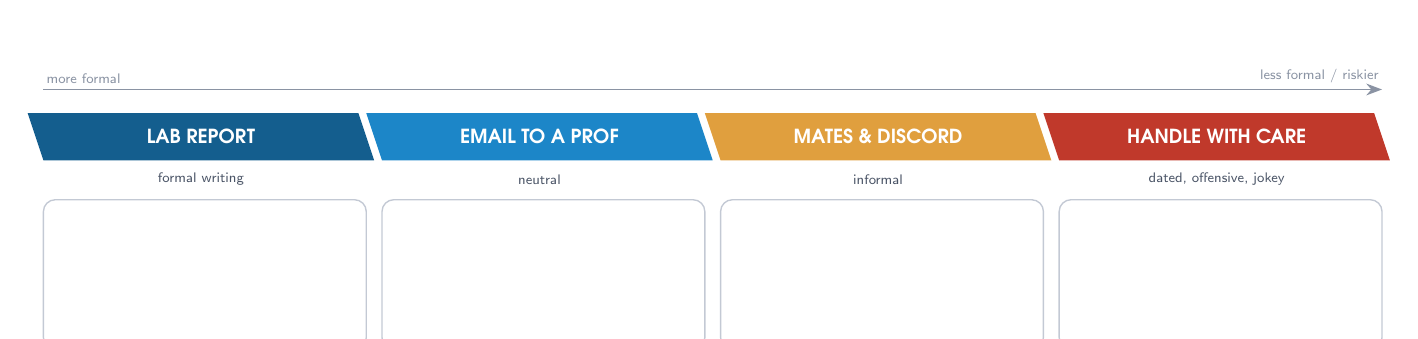
\begin{tikzpicture}[x=1mm,y=1mm]
\foreach \x/\c/\t/\s [count=\i] in {2/accentdark/LAB REPORT/formal writing, 45/accent/EMAIL TO A PROF/neutral, 88/vault/MATES \& DISCORD/informal, 131/bad/HANDLE WITH CARE/{dated, offensive, jokey}}{
  \fill[\c] (\x,24) -- (\x+42,24) -- (\x+40,30) -- (\x-2,30) -- cycle;
  \node[text=white,font=\hfont\bfseries\scriptsize] at (\x+20,27) {\t};
  \node[text=inksoft,font=\uifont\tiny] at (\x+20,21.6) {\s};
  \draw[line,line width=0.5pt,rounded corners=1.5mm] (\x,0) rectangle (\x+41,19);
}
\draw[-{Stealth[length=2mm]},mute,line width=0.6pt] (2,33) -- (172,33);
\node[anchor=south west,font=\uifont\tiny,text=mute,inner sep=1pt] at (2,33.4) {more formal};
\node[anchor=south east,font=\uifont\tiny,text=mute,inner sep=1pt] at (172,33.4) {less formal / riskier};
\end{tikzpicture}
\end{center}
\vspace{1mm}
\noindent{\small\textbf{Put band 1 to work.} Write two sentences for your Integrated Lab report using at least two band-1 words.}
\wlines{2}

% ---------------------------------------------------------------- Ex 16
\exhead[90mm]{16}{Transatlantic customs}{\tgL{B}{British}\,\tgL{F}{spelling}}{\mWrite\,\UK}
\instr{Much of your vault arrived from American dubs and subtitles. Time to clear it through British customs.}

\noindent{\hfont\bfseries\small\color{accent}A}\enspace{\small\textbf{Spelling passport.} Circle the British spelling. If both spellings are fine in the UK, circle both.}\par\vspace{1.4mm}
{\small\uifont\noindent\begin{tabular*}{\linewidth}{@{\extracolsep{\fill}}lll@{}}
\num{1} meager $\cdot$ meagre & \num{6} maneuver $\cdot$ manoeuvre & \num{11} specialty $\cdot$ speciality\\[1.3mm]
\num{2} savory $\cdot$ savoury & \num{7} installment $\cdot$ instalment & \num{12} jeopardize $\cdot$ jeopardise\\[1.3mm]
\num{3} skeptical $\cdot$ sceptical & \num{8} caliber $\cdot$ calibre & \num{13} spelled $\cdot$ spelt\\[1.3mm]
\num{4} smoldering $\cdot$ smouldering & \num{9} plowing $\cdot$ ploughing & \\[1.3mm]
\num{5} counseling $\cdot$ counselling & \num{10} unraveled $\cdot$ unravelled & \\
\end{tabular*}}

\par\vspace{2mm}\needsp{75mm}
\noindent{\hfont\bfseries\small\color{accent}B}\enspace{\small\textbf{Re-dub it for Lotte.} Jake from Ohio sent this to your Flemish friend Lotte. Rewrite the thirteen underlined bits the way someone in London would say or spell them.}\par\vspace{1.5mm}
\newcommand{\us}[2]{\underline{#2}\textsuperscript{\uifont\bfseries\tiny\color{accent}#1}}
\begin{tcolorbox}[enhanced,colback=accentsoft,colframe=accentsoft,boxrule=0pt,arc=3mm,left=4mm,right=4mm,top=2mm,bottom=2mm,fontupper=\small,
  sharp corners=southwest]
Hey Lotte! \us{1}{To make a long story short}, my new \us{2}{roommate} is driving me nuts. He’s been \us{3}{too big for his britches} since he became a \us{4}{full-fledged} member of the robotics team. Yesterday he left the \us{5}{trash} by the door all day, unplugged my laptop from the \us{6}{outlet} to charge his drone, and promised to \us{7}{do the dishes} \us{8}{from here on out}. Yeah, right. I wouldn’t touch his \us{9}{chili} with a \us{10}{ten-foot pole}, either. Anyway — cake at mine on Friday? I’ll cover it in \us{11}{sprinkles}, \us{12}{obvi}. It’s a \us{13}{vicious cycle}: I bake when I’m stressed, then I’m stressed because I baked.
\end{tcolorbox}
\vspace{1mm}
{\small\begin{multicols}{3}
\num{1} \blank[3.4cm]\par\vspace{1.7mm}\num{2} \blank[3.4cm]\par\vspace{1.7mm}\num{3} \blank[3.4cm]\par\vspace{1.7mm}\num{4} \blank[3.4cm]\par\vspace{1.7mm}\num{5} \blank[3.4cm]\par\vspace{1.7mm}
\num{6} \blank[3.4cm]\par\vspace{1.7mm}\num{7} \blank[3.4cm]\par\vspace{1.7mm}\num{8} \blank[3.4cm]\par\vspace{1.7mm}\num{9} \blank[3.4cm]\par\vspace{1.7mm}
\num{10} \blank[3.4cm]\par\vspace{1.7mm}\num{11} \blank[3.4cm]\par\vspace{1.7mm}\num{12} \blank[3.4cm]\par\vspace{1.7mm}\num{13} \blank[3.4cm]\par
\end{multicols}}
\vspace{1mm}
\needsp{45mm}
\noindent{\hfont\bfseries\small\color{accent}C}\enspace{\small\textbf{Same word, British meaning.} In a conversation in the UK, what does the underlined word most likely mean? Circle a or b.}\par\vspace{1.3mm}
\newcommand{\bq}[4]{\begin{minipage}[t]{\linewidth}\RaggedRight\num{#1} #2\par\hspace*{4mm}{\color{accent}a} #3 \enspace {\color{accent}b} #4\end{minipage}\par\vspace{1.6mm}}
{\small\noindent\begin{minipage}[t]{0.485\linewidth}
\bq{1}{“That plan is completely \ul{mad}.”}{angry}{crazy}
\bq{2}{“He slipped on the ice and landed on his \ul{bum}.”}{a homeless man}{his bottom}
\bq{3}{“Three lectures and a shift at work — I’m \ul{whacked}.”}{exhausted}{crazy}
\end{minipage}\hfill
\begin{minipage}[t]{0.485\linewidth}
\bq{4}{“The council has launched a new recycling \ul{scheme}.”}{a dishonest plot}{an official plan}
\bq{5}{“Can’t play tonight, sorry — my \ul{mocks} are next week.”}{practice exams}{jokes about me}
\bq{6}{“The \ul{landlord} pulled me a pint and asked about Brazil.”}{the owner of my flat}{the person who runs the pub}
\end{minipage}}

% ---------------------------------------------------------------- Ex 17
\newcommand{\hd}[1]{{\hfont\bfseries\normalsize\color{ink}\MakeUppercase{#1}}}
\newcommand{\hg}[1]{\mbox{{\uifont\bfseries\scriptsize\color{accent}#1}\kern1pt\textcolor{mute}{\rule[-0.4ex]{1.75cm}{0.5pt}}}}
\exhead[120mm]{17}{The Daily Vault}{\tgL{C}{collocation}\,\tgL{M}{meaning}\,\tgL{R}{register}}{\mWrite\,\UK}
\instr{British headlines are a language of their own: short, punchy words, no articles, present simple for things that already happened. Complete today’s front page with the words in the box (two are left over).}
\begin{wordbank}
\bank{soar, slashes, engulf, toll, hailed, thwarting, pledges, rampant, breach, disclose, looms, stalemate, bombshell, unveils, topple, unprecedented, farce, spree, plummet, cull}
\end{wordbank}
\vspace{1mm}
\begin{tcolorbox}[enhanced,colback=white,colframe=ink,boxrule=0.8pt,arc=0mm,left=3.5mm,right=3.5mm,top=2mm,bottom=2.5mm]
\begin{center}
{\fontfamily{pnc}\selectfont\bfseries\fontsize{30}{32}\selectfont THE DAILY VAULT}\par\vspace{0.6mm}
{\color{ink}\rule{\linewidth}{1.2pt}}\par\vspace{-1.4mm}{\color{ink}\rule{\linewidth}{0.4pt}}\par\vspace{0.4mm}
{\uifont\scriptsize\color{inksoft}Sunday 1 November 2026 \hfill Issue no.\ 925 \hfill Fictional, but very British}
\end{center}
\vspace{1.5mm}
\begin{minipage}[t]{0.485\linewidth}\RaggedRight
\hd{Bus fares to} \hg{1} \hd{as council} \hg{2} \hd{student discounts}\par\vspace{0.6mm}
{\footnotesize\color{inksoft}Leuven students face a winter of walking.}\par\vspace{2.6mm}
\hd{Flash floods} \hg{3} \hd{villages — death} \hg{4} \hd{rises to 12}\par\vspace{0.6mm}
{\footnotesize\color{inksoft}Rescue teams work through the night.}\par\vspace{2.6mm}
\hd{Student} \hg{5} \hd{as hero after} \hg{6} \hd{campus hack}\par\vspace{0.6mm}
{\footnotesize\color{inksoft}“I just noticed a weird log file,” says engineering fresher.}\par\vspace{2.6mm}
\hd{Mayor} \hg{7} \hd{to tackle} \hg{8} \hd{rents}\par\vspace{0.6mm}
{\footnotesize\color{inksoft}Landlords “disappointed”.}\par\vspace{2.6mm}
\hd{Uni admits data} \hg{9}\hd{, refuses to} \hg{10} \hd{how many affected}\par
\end{minipage}\hfill{\color{line}\vrule width 0.5pt}\hfill
\begin{minipage}[t]{0.47\linewidth}\RaggedRight
\hd{Rail strike} \hg{11} \hd{as pay talks end in} \hg{12}\par\vspace{0.6mm}
{\footnotesize\color{inksoft}Commuters told to work from home.}\par\vspace{2.6mm}
\hg{13} \hd{report: care homes accused of decades of neglect}\par\vspace{2.6mm}
\hd{Government} \hg{14} \hd{plan to cut energy bills}\par\vspace{2.6mm}
\hd{Amateurs} \hg{15} \hd{champions in} \hg{16} \hd{cup upset}\par\vspace{0.6mm}
{\footnotesize\color{inksoft}Fourth-tier side stun the holders 2--1.}\par\vspace{2.6mm}
\hd{Trial descends into} \hg{17} \hd{as judge nods off}\par\vspace{2.6mm}
\hd{Teen’s £3,000 gaming} \hg{18} \hd{on mum’s card}\par
\end{minipage}
\end{tcolorbox}
\vspace{1mm}
\noindent{\hfont\bfseries\small\color{accent}B}\enspace{\small\textbf{Headline decoder.}}\par\vspace{1mm}
{\small\RaggedRight
\num{a} Headline 1 says \emph{TO} + verb. What does that tell you about time?\wline
\num{b} The cup headline uses the present simple. When did the match happen?\wline
\num{c} Rewrite the mayor’s headline as a normal sentence, with articles and a full verb phrase.\wline}

% =====================================================================
% PART 7 — LET LOOSE
% =====================================================================
\partbanner{PART 7}{LET LOOSE}{Stop holding back: explain, improvise, tell stories. This is where the stutter goes.}

% ---------------------------------------------------------------- Ex 18
\newcommand{\taboo}[4]{%
  \begin{tcolorbox}[enhanced,colback=white,colframe=ink,boxrule=0.6pt,arc=2mm,left=2.5mm,right=2.5mm,top=1.4mm,bottom=1.4mm,
    title={\hfont\bfseries\normalsize\MakeUppercase{#1}},halign title=center,coltitle=white,colbacktitle=accent,toptitle=0.8mm,bottomtitle=0.8mm,
    fontupper=\small\uifont,halign=center,height=14.5mm,valign=center]
  {\color{bad}\ding{55}}\,#2\enspace{\color{bad}\ding{55}}\,#3\enspace{\color{bad}\ding{55}}\,#4
  \end{tcolorbox}}
\exhead[105mm]{18}{Taboo}{\tgL{M}{meaning}}{\mSpeak\,\mTimed}
\instr{Explain each word out loud in under 30 seconds — as if to a classmate who has never heard it — \emph{without} saying the word itself or the three forbidden words. Record yourself; if you freeze, that word goes on your comeback list. This trains exactly what the break took away: talking your way around a gap without stopping.}
\vspace{1mm}
\noindent\begin{minipage}[t]{0.32\linewidth}
\taboo{heirloom}{family}{old}{valuable}
\taboo{grudge}{angry}{forgive}{past}
\taboo{cliffhanger}{end}{episode}{suspense}
\taboo{knack}{skill}{talent}{good at}
\end{minipage}\hfill
\begin{minipage}[t]{0.32\linewidth}
\taboo{rip-off}{expensive}{price}{cheat}
\taboo{sabbatical}{break}{year}{work}
\taboo{pep talk}{motivate}{speech}{coach}
\taboo{tinfoil hat}{conspiracy}{crazy}{aluminium}
\end{minipage}\hfill
\begin{minipage}[t]{0.32\linewidth}
\taboo{shoo-in}{win}{certain}{favourite}
\taboo{whereabouts}{where}{place}{location}
\taboo{trump card}{card}{advantage}{secret}
\taboo{landlord}{rent}{house}{owner}
\end{minipage}

% ---------------------------------------------------------------- Ex 19
\newcommand{\dm}[1]{\tikz[baseline=(c.base)]{\node[inner xsep=3pt,inner ysep=2pt,fill=vaultsoft,rounded corners=2pt,font=\uifont\small](c){\cbox\enspace #1};}}
\newcommand{\hs}[2]{\num{#1}\enspace #2\par\vspace{1.5mm}}
\exhead[95mm]{19}{Hot seat}{\tgL{I}{idioms}\,\tgL{R}{register}\,\tgL{B}{British}}{\mSpeak\,\mTimed}
\instr{Answer each question out loud for 30--45 seconds. Two rules: use the \textbf{bold} chunk, and slip in one \emph{discourse marker} from the deck (tick it; by the end, use all eight — markers buy you thinking time without sounding stuck). Record your three best answers and count the pauses longer than two seconds. Do the same on Day 7 of your rematch: fewer pauses is the whole point.}
\vspace{0.5mm}
\begin{center}
\dm{as far as I’m concerned}\enspace\dm{be that as it may}\enspace\dm{to cut a long story short}\enspace\dm{by all accounts}\\[1.6mm]
\dm{all along}\enspace\dm{every now and then}\enspace\dm{frankly}\enspace\dm{merely}
\end{center}
\vspace{1mm}
{\small\begin{multicols}{2}\RaggedRight
\hs{1}{What’s something in Leuven that’s a total \textbf{rip-off}?}
\hs{2}{Tell me about a plan of yours that \textbf{backfired}.}
\hs{3}{What’s a skill you want to \textbf{hone} this year — and how?}
\hs{4}{When did you last \textbf{bite off more than you could chew}?}
\hs{5}{What’s your \textbf{trump card} in an exam — or in a ranked match?}
\hs{6}{What’s something you simply \textbf{can’t abide}?}
\hs{7}{Describe a \textbf{lucky break} you’ve had.}
\hs{8}{Who did you \textbf{hold in high esteem} as a kid, and why?}
\hs{9}{Have you ever been \textbf{caught red-handed}? Doing what?}
\hs{10}{What would make you \textbf{call it quits} on a game for good?}
\hs{11}{What has turned out to be \textbf{a blessing in disguise} for you?}
\hs{12}{What are you \textbf{keen on} at the moment? (Say it the British way: \emph{I’m really keen on\ldots})}
\end{multicols}}


% ---------------------------------------------------------------- Ex 20
\newcommand{\diceface}[1]{\tikz[x=1mm,y=1mm,baseline=-0.8ex]{\draw[ink,rounded corners=0.6mm,line width=0.55pt,fill=white] (-2.3,-2.3) rectangle (2.3,2.3);
  \ifcase#1\or \fill (0,0) circle (0.42);
  \or \fill (-1.1,1.1) circle (0.42); \fill (1.1,-1.1) circle (0.42);
  \or \fill (-1.1,1.1) circle (0.42); \fill (0,0) circle (0.42); \fill (1.1,-1.1) circle (0.42);
  \or \fill (-1.1,1.1) circle (0.42); \fill (1.1,1.1) circle (0.42); \fill (-1.1,-1.1) circle (0.42); \fill (1.1,-1.1) circle (0.42);
  \or \fill (-1.1,1.1) circle (0.42); \fill (1.1,1.1) circle (0.42); \fill (0,0) circle (0.42); \fill (-1.1,-1.1) circle (0.42); \fill (1.1,-1.1) circle (0.42);
  \or \fill (-1.1,1.1) circle (0.42); \fill (1.1,1.1) circle (0.42); \fill (-1.1,0) circle (0.42); \fill (1.1,0) circle (0.42); \fill (-1.1,-1.1) circle (0.42); \fill (1.1,-1.1) circle (0.42);
  \fi}}
\exhead[150mm]{20}{Loot-box mini-saga}{\tgL{C}{collocation}\,\tgL{M}{meaning}}{\mDice\,\mWrite}
\instr{Roll two dice five times: first die = row, second die = column. (No dice? Use any online dice roller.) Then write a \textbf{mini-saga}: a complete story in \emph{exactly} 50 words — not 49, not 51; the title doesn’t count — using all five words you rolled. Forms can change (\emph{backfire} \arr{} \emph{backfired}). Topic ideas: \emph{my first week in Leuven} \mdot{} \emph{the experiment that went wrong} \mdot{} \emph{the match we threw} \mdot{} \emph{a message I shouldn’t have sent}.}
\vspace{1mm}
\begin{center}
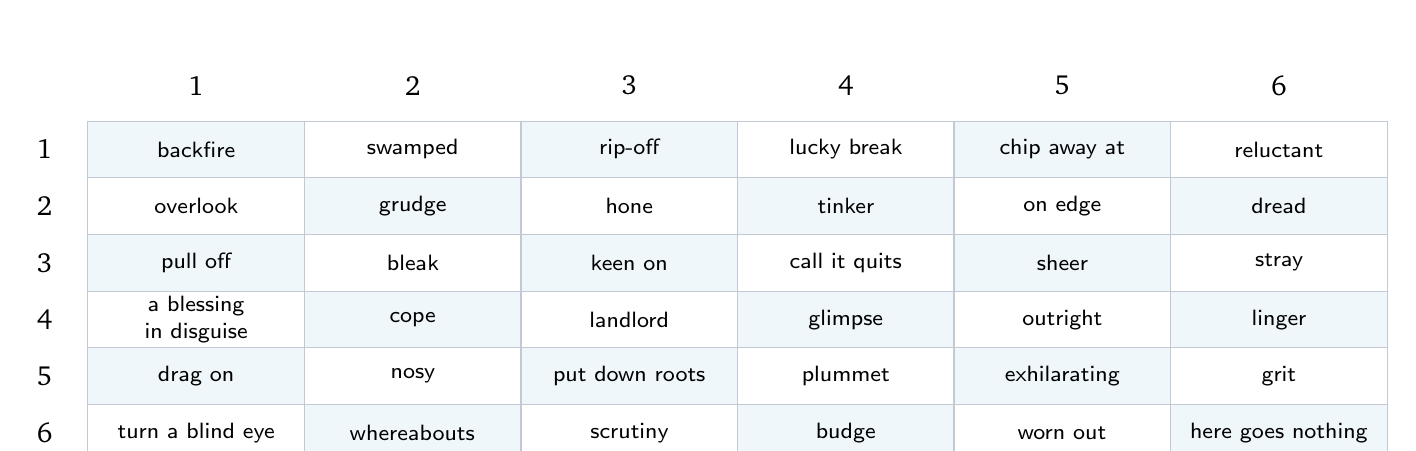
\begin{tikzpicture}[x=1mm,y=-1mm]
\def\cw{27.5} \def\ch{7.2}
\foreach \c in {1,...,6}{\node at (8+\c*\cw-\cw/2,-4.5) {\diceface{\c}};}
\foreach \r in {1,...,6}{\node at (2.5,\r*\ch-\ch/2) {\diceface{\r}};}
\foreach \r/\row in {1/{backfire,swamped,rip-off,lucky break,chip away at,reluctant},
                     2/{overlook,grudge,hone,tinker,on edge,dread},
                     3/{pull off,bleak,keen on,call it quits,sheer,stray},
                     4/{a blessing in disguise,cope,landlord,glimpse,outright,linger},
                     5/{drag on,nosy,put down roots,plummet,exhilarating,grit},
                     6/{turn a blind eye,whereabouts,scrutiny,budge,worn out,here goes nothing}}{
  \foreach \w [count=\c] in \row {
    \pgfmathsetmacro\fillc{mod(\r+\c,2)==0 ? 1 : 0}
    \ifdim\fillc pt=1pt \fill[accent!7] (8+\c*\cw-\cw,\r*\ch-\ch) rectangle (8+\c*\cw,\r*\ch); \fi
    \draw[line,line width=0.4pt] (8+\c*\cw-\cw,\r*\ch-\ch) rectangle (8+\c*\cw,\r*\ch);
    \node[font=\uifont\footnotesize,text width=25mm,align=center] at (8+\c*\cw-\cw/2,\r*\ch-\ch/2) {\w};
  }}
\end{tikzpicture}
\end{center}
\vspace{1mm}
\noindent{\small\textbf{Your loot:}\enspace\num{1}~\blank[2.3cm]\enspace\num{2}~\blank[2.3cm]\enspace\num{3}~\blank[2.3cm]\enspace\num{4}~\blank[2.3cm]\enspace\num{5}~\blank[2.3cm]}
\par\vspace{2.5mm}
\noindent{\small\textbf{Title:}}\enspace\wfill
\wlines{6}
\noindent{\small\textbf{Word count:}}\enspace\lbox{12mm}\enspace{\small\color{inksoft}\hfill Check: \cbox{} exactly 50 \enspace\cbox{} all five words \enspace\cbox{} forms and partners right (\emph{tinker \textbf{with}}, \emph{keen \textbf{on}})}


% =====================================================================
% RUNDOWN
% =====================================================================
\newpage
\noindent
\begin{tikzpicture}
  \path[use as bounding box] (0,0) rectangle (\linewidth,-21.5mm);
  \fill[ink] (0,0) -- (\linewidth,0) -- (\linewidth-9mm,-15mm) -- (0,-15mm) -- cycle;
  \fill[vault] (0,0) rectangle (3.2mm,-15mm);
  \fill[vault] (\linewidth-5mm,0) -- (\linewidth,0) -- (\linewidth-9mm,-15mm) -- (\linewidth-14mm,-15mm) -- cycle;
  \node[anchor=west,font=\hfont\bfseries\footnotesize,text=vault] at (7.5mm,-4.6mm) {AFTER THE MATCH};
  \node[anchor=west,font=\hfont\bfseries\fontsize{21}{23}\selectfont,text=white] at (7mm,-10.3mm) {RUNDOWN};
  \node[anchor=north west,font=\itshape\small,text=inksoft,inner sep=0pt] at (0.4mm,-17.6mm) {A summary of the main points (your JJK card). Find your weak spots, plan the rematch, let the rest go.};
\end{tikzpicture}
\par\vspace{2mm}

\noindent{\hfont\bfseries\small\color{ink}1 \enspace YOUR REDS, BY TAG}\enspace{\small\color{inksoft}— colour one square for every red answer (wrong, then corrected). Two or more in a row = your next focus.}\par\vspace{1.5mm}
\noindent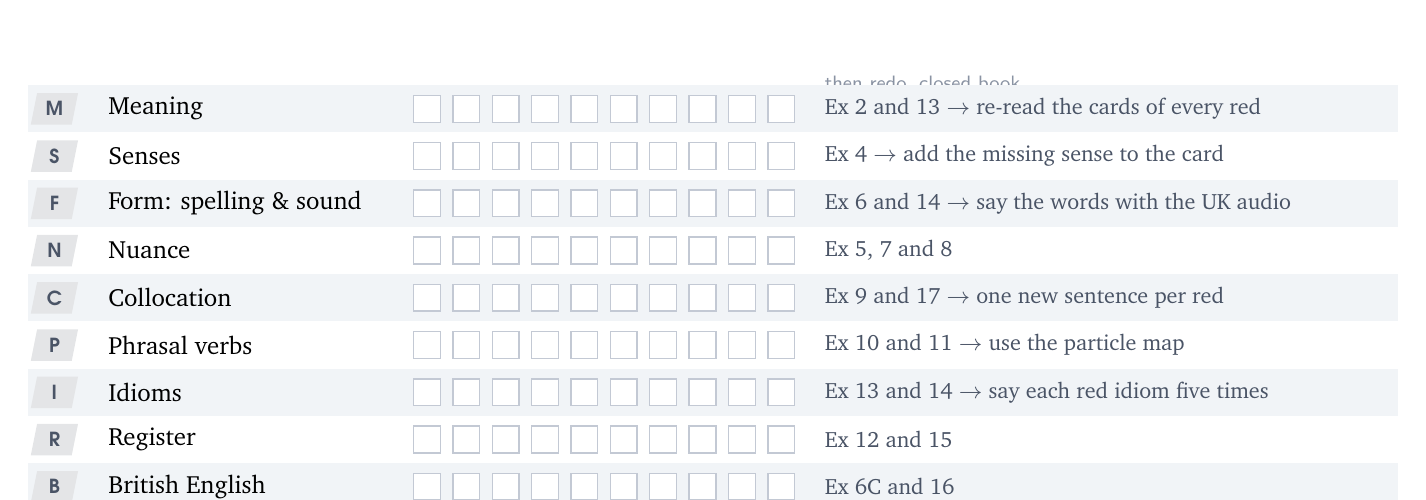
\begin{tikzpicture}[x=1mm,y=-1mm]
\node[anchor=west,font=\uifont\scriptsize,text=mute] at (100,-3.2) {then redo, closed book};
\fill[paper] (0,-3.00) rectangle (174,3.00);
\fill[ink!12] (1.2,-2.00) -- (6.4,-2.00) -- (5.6,2.00) -- (0.4,2.00) -- cycle;
\node[font=\hfont\bfseries\scriptsize,text=inksoft] at (3.4,0.00) {M};
\node[anchor=west,font=\small] at (9,0.00) {Meaning};
\draw[line,line width=0.5pt,fill=white] (49.00,-1.70) rectangle +(3.4,3.4);
\draw[line,line width=0.5pt,fill=white] (54.00,-1.70) rectangle +(3.4,3.4);
\draw[line,line width=0.5pt,fill=white] (59.00,-1.70) rectangle +(3.4,3.4);
\draw[line,line width=0.5pt,fill=white] (64.00,-1.70) rectangle +(3.4,3.4);
\draw[line,line width=0.5pt,fill=white] (69.00,-1.70) rectangle +(3.4,3.4);
\draw[line,line width=0.5pt,fill=white] (74.00,-1.70) rectangle +(3.4,3.4);
\draw[line,line width=0.5pt,fill=white] (79.00,-1.70) rectangle +(3.4,3.4);
\draw[line,line width=0.5pt,fill=white] (84.00,-1.70) rectangle +(3.4,3.4);
\draw[line,line width=0.5pt,fill=white] (89.00,-1.70) rectangle +(3.4,3.4);
\draw[line,line width=0.5pt,fill=white] (94.00,-1.70) rectangle +(3.4,3.4);
\node[anchor=west,font=\footnotesize,text=inksoft] at (100,0.00) {Ex 2 and 13 \arr{} re-read the cards of every red};
\fill[ink!12] (1.2,4.00) -- (6.4,4.00) -- (5.6,8.00) -- (0.4,8.00) -- cycle;
\node[font=\hfont\bfseries\scriptsize,text=inksoft] at (3.4,6.00) {S};
\node[anchor=west,font=\small] at (9,6.00) {Senses};
\draw[line,line width=0.5pt,fill=white] (49.00,4.30) rectangle +(3.4,3.4);
\draw[line,line width=0.5pt,fill=white] (54.00,4.30) rectangle +(3.4,3.4);
\draw[line,line width=0.5pt,fill=white] (59.00,4.30) rectangle +(3.4,3.4);
\draw[line,line width=0.5pt,fill=white] (64.00,4.30) rectangle +(3.4,3.4);
\draw[line,line width=0.5pt,fill=white] (69.00,4.30) rectangle +(3.4,3.4);
\draw[line,line width=0.5pt,fill=white] (74.00,4.30) rectangle +(3.4,3.4);
\draw[line,line width=0.5pt,fill=white] (79.00,4.30) rectangle +(3.4,3.4);
\draw[line,line width=0.5pt,fill=white] (84.00,4.30) rectangle +(3.4,3.4);
\draw[line,line width=0.5pt,fill=white] (89.00,4.30) rectangle +(3.4,3.4);
\draw[line,line width=0.5pt,fill=white] (94.00,4.30) rectangle +(3.4,3.4);
\node[anchor=west,font=\footnotesize,text=inksoft] at (100,6.00) {Ex 4 \arr{} add the missing sense to the card};
\fill[paper] (0,9.00) rectangle (174,15.00);
\fill[ink!12] (1.2,10.00) -- (6.4,10.00) -- (5.6,14.00) -- (0.4,14.00) -- cycle;
\node[font=\hfont\bfseries\scriptsize,text=inksoft] at (3.4,12.00) {F};
\node[anchor=west,font=\small] at (9,12.00) {Form: spelling \& sound};
\draw[line,line width=0.5pt,fill=white] (49.00,10.30) rectangle +(3.4,3.4);
\draw[line,line width=0.5pt,fill=white] (54.00,10.30) rectangle +(3.4,3.4);
\draw[line,line width=0.5pt,fill=white] (59.00,10.30) rectangle +(3.4,3.4);
\draw[line,line width=0.5pt,fill=white] (64.00,10.30) rectangle +(3.4,3.4);
\draw[line,line width=0.5pt,fill=white] (69.00,10.30) rectangle +(3.4,3.4);
\draw[line,line width=0.5pt,fill=white] (74.00,10.30) rectangle +(3.4,3.4);
\draw[line,line width=0.5pt,fill=white] (79.00,10.30) rectangle +(3.4,3.4);
\draw[line,line width=0.5pt,fill=white] (84.00,10.30) rectangle +(3.4,3.4);
\draw[line,line width=0.5pt,fill=white] (89.00,10.30) rectangle +(3.4,3.4);
\draw[line,line width=0.5pt,fill=white] (94.00,10.30) rectangle +(3.4,3.4);
\node[anchor=west,font=\footnotesize,text=inksoft] at (100,12.00) {Ex 6 and 14 \arr{} say the words with the UK audio};
\fill[ink!12] (1.2,16.00) -- (6.4,16.00) -- (5.6,20.00) -- (0.4,20.00) -- cycle;
\node[font=\hfont\bfseries\scriptsize,text=inksoft] at (3.4,18.00) {N};
\node[anchor=west,font=\small] at (9,18.00) {Nuance};
\draw[line,line width=0.5pt,fill=white] (49.00,16.30) rectangle +(3.4,3.4);
\draw[line,line width=0.5pt,fill=white] (54.00,16.30) rectangle +(3.4,3.4);
\draw[line,line width=0.5pt,fill=white] (59.00,16.30) rectangle +(3.4,3.4);
\draw[line,line width=0.5pt,fill=white] (64.00,16.30) rectangle +(3.4,3.4);
\draw[line,line width=0.5pt,fill=white] (69.00,16.30) rectangle +(3.4,3.4);
\draw[line,line width=0.5pt,fill=white] (74.00,16.30) rectangle +(3.4,3.4);
\draw[line,line width=0.5pt,fill=white] (79.00,16.30) rectangle +(3.4,3.4);
\draw[line,line width=0.5pt,fill=white] (84.00,16.30) rectangle +(3.4,3.4);
\draw[line,line width=0.5pt,fill=white] (89.00,16.30) rectangle +(3.4,3.4);
\draw[line,line width=0.5pt,fill=white] (94.00,16.30) rectangle +(3.4,3.4);
\node[anchor=west,font=\footnotesize,text=inksoft] at (100,18.00) {Ex 5, 7 and 8};
\fill[paper] (0,21.00) rectangle (174,27.00);
\fill[ink!12] (1.2,22.00) -- (6.4,22.00) -- (5.6,26.00) -- (0.4,26.00) -- cycle;
\node[font=\hfont\bfseries\scriptsize,text=inksoft] at (3.4,24.00) {C};
\node[anchor=west,font=\small] at (9,24.00) {Collocation};
\draw[line,line width=0.5pt,fill=white] (49.00,22.30) rectangle +(3.4,3.4);
\draw[line,line width=0.5pt,fill=white] (54.00,22.30) rectangle +(3.4,3.4);
\draw[line,line width=0.5pt,fill=white] (59.00,22.30) rectangle +(3.4,3.4);
\draw[line,line width=0.5pt,fill=white] (64.00,22.30) rectangle +(3.4,3.4);
\draw[line,line width=0.5pt,fill=white] (69.00,22.30) rectangle +(3.4,3.4);
\draw[line,line width=0.5pt,fill=white] (74.00,22.30) rectangle +(3.4,3.4);
\draw[line,line width=0.5pt,fill=white] (79.00,22.30) rectangle +(3.4,3.4);
\draw[line,line width=0.5pt,fill=white] (84.00,22.30) rectangle +(3.4,3.4);
\draw[line,line width=0.5pt,fill=white] (89.00,22.30) rectangle +(3.4,3.4);
\draw[line,line width=0.5pt,fill=white] (94.00,22.30) rectangle +(3.4,3.4);
\node[anchor=west,font=\footnotesize,text=inksoft] at (100,24.00) {Ex 9 and 17 \arr{} one new sentence per red};
\fill[ink!12] (1.2,28.00) -- (6.4,28.00) -- (5.6,32.00) -- (0.4,32.00) -- cycle;
\node[font=\hfont\bfseries\scriptsize,text=inksoft] at (3.4,30.00) {P};
\node[anchor=west,font=\small] at (9,30.00) {Phrasal verbs};
\draw[line,line width=0.5pt,fill=white] (49.00,28.30) rectangle +(3.4,3.4);
\draw[line,line width=0.5pt,fill=white] (54.00,28.30) rectangle +(3.4,3.4);
\draw[line,line width=0.5pt,fill=white] (59.00,28.30) rectangle +(3.4,3.4);
\draw[line,line width=0.5pt,fill=white] (64.00,28.30) rectangle +(3.4,3.4);
\draw[line,line width=0.5pt,fill=white] (69.00,28.30) rectangle +(3.4,3.4);
\draw[line,line width=0.5pt,fill=white] (74.00,28.30) rectangle +(3.4,3.4);
\draw[line,line width=0.5pt,fill=white] (79.00,28.30) rectangle +(3.4,3.4);
\draw[line,line width=0.5pt,fill=white] (84.00,28.30) rectangle +(3.4,3.4);
\draw[line,line width=0.5pt,fill=white] (89.00,28.30) rectangle +(3.4,3.4);
\draw[line,line width=0.5pt,fill=white] (94.00,28.30) rectangle +(3.4,3.4);
\node[anchor=west,font=\footnotesize,text=inksoft] at (100,30.00) {Ex 10 and 11 \arr{} use the particle map};
\fill[paper] (0,33.00) rectangle (174,39.00);
\fill[ink!12] (1.2,34.00) -- (6.4,34.00) -- (5.6,38.00) -- (0.4,38.00) -- cycle;
\node[font=\hfont\bfseries\scriptsize,text=inksoft] at (3.4,36.00) {I};
\node[anchor=west,font=\small] at (9,36.00) {Idioms};
\draw[line,line width=0.5pt,fill=white] (49.00,34.30) rectangle +(3.4,3.4);
\draw[line,line width=0.5pt,fill=white] (54.00,34.30) rectangle +(3.4,3.4);
\draw[line,line width=0.5pt,fill=white] (59.00,34.30) rectangle +(3.4,3.4);
\draw[line,line width=0.5pt,fill=white] (64.00,34.30) rectangle +(3.4,3.4);
\draw[line,line width=0.5pt,fill=white] (69.00,34.30) rectangle +(3.4,3.4);
\draw[line,line width=0.5pt,fill=white] (74.00,34.30) rectangle +(3.4,3.4);
\draw[line,line width=0.5pt,fill=white] (79.00,34.30) rectangle +(3.4,3.4);
\draw[line,line width=0.5pt,fill=white] (84.00,34.30) rectangle +(3.4,3.4);
\draw[line,line width=0.5pt,fill=white] (89.00,34.30) rectangle +(3.4,3.4);
\draw[line,line width=0.5pt,fill=white] (94.00,34.30) rectangle +(3.4,3.4);
\node[anchor=west,font=\footnotesize,text=inksoft] at (100,36.00) {Ex 13 and 14 \arr{} say each red idiom five times};
\fill[ink!12] (1.2,40.00) -- (6.4,40.00) -- (5.6,44.00) -- (0.4,44.00) -- cycle;
\node[font=\hfont\bfseries\scriptsize,text=inksoft] at (3.4,42.00) {R};
\node[anchor=west,font=\small] at (9,42.00) {Register};
\draw[line,line width=0.5pt,fill=white] (49.00,40.30) rectangle +(3.4,3.4);
\draw[line,line width=0.5pt,fill=white] (54.00,40.30) rectangle +(3.4,3.4);
\draw[line,line width=0.5pt,fill=white] (59.00,40.30) rectangle +(3.4,3.4);
\draw[line,line width=0.5pt,fill=white] (64.00,40.30) rectangle +(3.4,3.4);
\draw[line,line width=0.5pt,fill=white] (69.00,40.30) rectangle +(3.4,3.4);
\draw[line,line width=0.5pt,fill=white] (74.00,40.30) rectangle +(3.4,3.4);
\draw[line,line width=0.5pt,fill=white] (79.00,40.30) rectangle +(3.4,3.4);
\draw[line,line width=0.5pt,fill=white] (84.00,40.30) rectangle +(3.4,3.4);
\draw[line,line width=0.5pt,fill=white] (89.00,40.30) rectangle +(3.4,3.4);
\draw[line,line width=0.5pt,fill=white] (94.00,40.30) rectangle +(3.4,3.4);
\node[anchor=west,font=\footnotesize,text=inksoft] at (100,42.00) {Ex 12 and 15};
\fill[paper] (0,45.00) rectangle (174,51.00);
\fill[ink!12] (1.2,46.00) -- (6.4,46.00) -- (5.6,50.00) -- (0.4,50.00) -- cycle;
\node[font=\hfont\bfseries\scriptsize,text=inksoft] at (3.4,48.00) {B};
\node[anchor=west,font=\small] at (9,48.00) {British English};
\draw[line,line width=0.5pt,fill=white] (49.00,46.30) rectangle +(3.4,3.4);
\draw[line,line width=0.5pt,fill=white] (54.00,46.30) rectangle +(3.4,3.4);
\draw[line,line width=0.5pt,fill=white] (59.00,46.30) rectangle +(3.4,3.4);
\draw[line,line width=0.5pt,fill=white] (64.00,46.30) rectangle +(3.4,3.4);
\draw[line,line width=0.5pt,fill=white] (69.00,46.30) rectangle +(3.4,3.4);
\draw[line,line width=0.5pt,fill=white] (74.00,46.30) rectangle +(3.4,3.4);
\draw[line,line width=0.5pt,fill=white] (79.00,46.30) rectangle +(3.4,3.4);
\draw[line,line width=0.5pt,fill=white] (84.00,46.30) rectangle +(3.4,3.4);
\draw[line,line width=0.5pt,fill=white] (89.00,46.30) rectangle +(3.4,3.4);
\draw[line,line width=0.5pt,fill=white] (94.00,46.30) rectangle +(3.4,3.4);
\node[anchor=west,font=\footnotesize,text=inksoft] at (100,48.00) {Ex 6C and 16};
\end{tikzpicture}
\par\vspace{3mm}

\noindent{\hfont\bfseries\small\color{ink}2 \enspace MY COMEBACK WORDS}\enspace{\small\color{inksoft}— the reds that hurt most. A new sentence about \emph{your} life makes them stick.}\par\vspace{4mm}
\noindent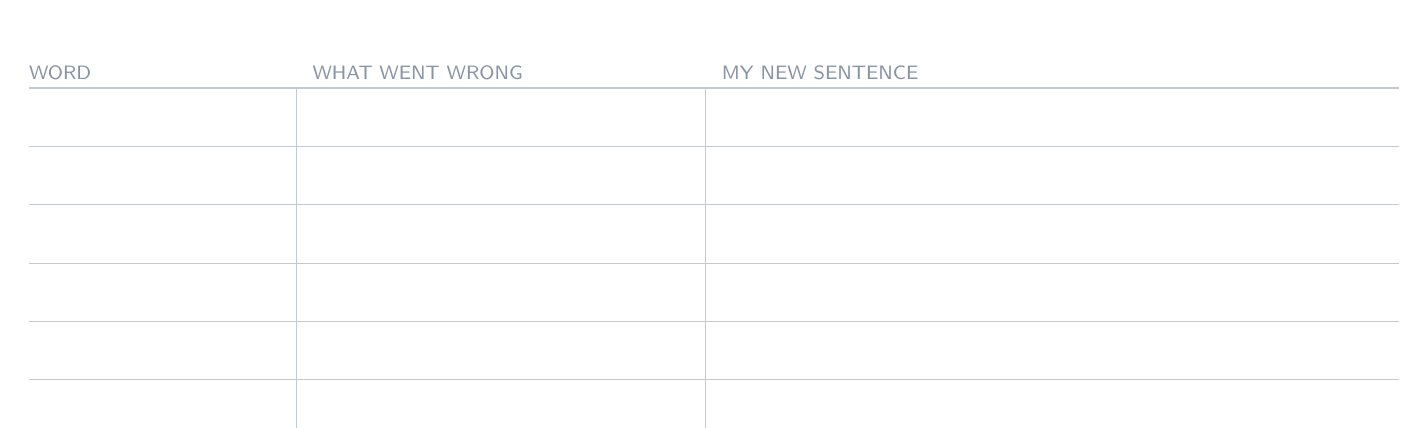
\begin{tikzpicture}[x=1mm,y=-1mm]
\node[anchor=south west,font=\uifont\scriptsize,text=mute,inner sep=0pt] at (0,-1) {WORD};
\node[anchor=south west,font=\uifont\scriptsize,text=mute,inner sep=0pt] at (36,-1) {WHAT WENT WRONG};
\node[anchor=south west,font=\uifont\scriptsize,text=mute,inner sep=0pt] at (88,-1) {MY NEW SENTENCE};
\draw[line,line width=0.6pt] (0,0.00) -- (174,0.00);
\draw[line,line width=0.4pt] (0,7.40) -- (174,7.40);
\draw[line,line width=0.4pt] (0,14.80) -- (174,14.80);
\draw[line,line width=0.4pt] (0,22.20) -- (174,22.20);
\draw[line,line width=0.4pt] (0,29.60) -- (174,29.60);
\draw[line,line width=0.4pt] (0,37.00) -- (174,37.00);
\draw[line,line width=0.4pt] (0,44.40) -- (174,44.40);
\draw[line,line width=0.4pt] (34,0) -- (34,44.40);
\draw[line,line width=0.4pt] (86,0) -- (86,44.40);
\end{tikzpicture}
\par\vspace{3mm}

\noindent{\hfont\bfseries\small\color{ink}3 \enspace REMATCH SCHEDULE}\enspace{\small\color{inksoft}— spaced retrieval: each comeback is a little harder, and that is exactly why it works.}\par\vspace{2mm}
\begin{center}
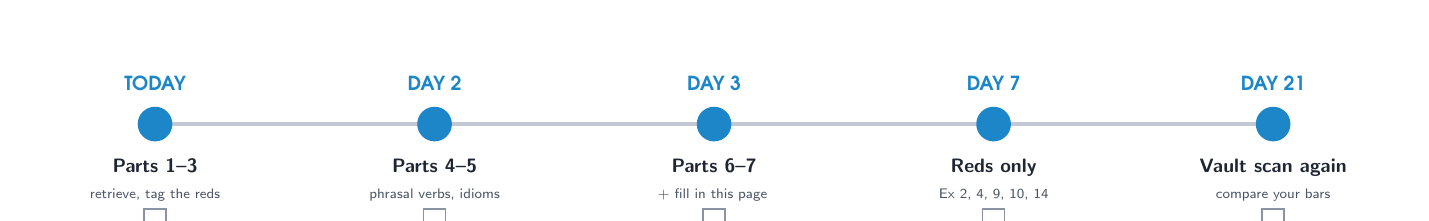
\begin{tikzpicture}[x=1mm,y=1mm]
\draw[line,line width=1.2pt] (16,0) -- (158,0);
\foreach \x/\d/\t/\s in {16/TODAY/Parts 1--3/{retrieve, tag the reds},
                         51.5/DAY 2/Parts 4--5/{phrasal verbs, idioms},
                         87/DAY 3/Parts 6--7/{+ fill in this page},
                         122.5/DAY 7/Reds only/{Ex 2, 4, 9, 10, 14},
                         158/DAY 21/Vault scan again/{compare your bars}}{
  \fill[accent] (\x,0) circle (2.2);
  \node[anchor=south,font=\hfont\bfseries\scriptsize,text=accent] at (\x,3) {\d};
  \node[anchor=north,font=\uifont\bfseries\scriptsize,text=ink,align=center] at (\x,-3.2) {\t};
  \node[anchor=north,font=\uifont\tiny,text=inksoft,align=center,text width=30mm] at (\x,-7) {\s};
  \draw[mute,line width=0.5pt] (\x-1.4,-13.6) rectangle (\x+1.4,-10.8);
}
\end{tikzpicture}
\end{center}
\vspace{1mm}
\begin{vaultbox}
\vaultI\enspace\textbf{Vault homework (5 minutes).} Open the card behind every red and add \texttt{recall} to its \texttt{tags:} list. Before each rematch, search \texttt{tag:\#recall} in Obsidian and read only those cards. When a word has survived Day 21, remove the tag — it has earned it.
\end{vaultbox}
\vspace{1mm}

\noindent{\hfont\bfseries\small\color{ink}4 \enspace LET IT GO}\enspace{\small\color{inksoft}— tier C: recognise these if they come up, but don’t spend review time on them.}\par\vspace{1.5mm}
\newcommand{\letgo}[1]{\tikz[baseline=(c.base)]{\node[inner xsep=2.6pt,inner ysep=1.6pt,draw=line,rounded corners=1.5pt,font=\uifont\footnotesize,text=inksoft](c){#1};}}
\noindent{\RaggedRight\letgo{tarnation}\hspace{2pt plus 2pt}\allowbreak\letgo{oogey}\hspace{2pt plus 2pt}\allowbreak\letgo{yeller}\hspace{2pt plus 2pt}\allowbreak\letgo{whippersnapper}\hspace{2pt plus 2pt}\allowbreak\letgo{even-steven}\hspace{2pt plus 2pt}\allowbreak\letgo{doughboy}\hspace{2pt plus 2pt}\allowbreak\letgo{nickel}\hspace{2pt plus 2pt}\allowbreak\letgo{batter up}\hspace{2pt plus 2pt}\allowbreak\letgo{cruller}\hspace{2pt plus 2pt}\allowbreak\letgo{eggrolls}\hspace{2pt plus 2pt}\allowbreak\letgo{calamari}\hspace{2pt plus 2pt}\allowbreak\letgo{cephalopod}\hspace{2pt plus 2pt}\allowbreak\letgo{soybean}\hspace{2pt plus 2pt}\allowbreak\letgo{shortcake}\hspace{2pt plus 2pt}\allowbreak\letgo{thee}\hspace{2pt plus 2pt}\allowbreak\letgo{whence}\hspace{2pt plus 2pt}\allowbreak\letgo{beseech}\hspace{2pt plus 2pt}\allowbreak\letgo{eyeholes}\hspace{2pt plus 2pt}\allowbreak\letgo{slap kick}\hspace{2pt plus 2pt}\allowbreak\letgo{knick}\hspace{2pt plus 2pt}\allowbreak\letgo{rash guard}\hspace{2pt plus 2pt}\allowbreak\letgo{the needles and thread\ldots}\par}
\vspace{1mm}
{\footnotesize\color{inksoft}Why these? Dub-only or archaic slang, food and animal words you will never need to produce, and lines that only make sense inside one scene. Your brain has better things to do in exam season.}

\end{document}
